% ============================================================================
%  Regime-Adaptive Pairs Trading with Robust Kalman Filtering
%  IEEE Access Format
% ============================================================================
\IfFileExists{ieeeaccess.cls}{
\documentclass{ieeeaccess}
}{
\documentclass{IEEEtran}
}
\IEEEoverridecommandlockouts

\usepackage[utf8]{inputenc}
\usepackage[T1]{fontenc}
\usepackage{amsmath,amssymb,amsfonts}
\usepackage{algorithmic}
\usepackage{algorithm}
\usepackage{graphicx}
\usepackage{textcomp}
\usepackage{booktabs}
\usepackage{multirow}
\usepackage{hyperref}
\usepackage{xcolor}
\usepackage{tabularx}
\usepackage{subcaption}
\usepackage{float}
\usepackage{colortbl}   % for \rowcolor in walk-forward table

\hypersetup{
    colorlinks=true,
    linkcolor=blue!70!black,
    citecolor=blue!70!black,
    urlcolor=blue!70!black,
}

\graphicspath{{figures/}}

\def\BibTeX{{\rm B\kern-.05em{\sc i\kern-.025em b}\kern-.08em
    T\kern-.1667em\lower.7ex\hbox{E}\kern-.125emX}}

\begin{document}

\title{Regime-Adaptive Pairs Trading with Robust Kalman Filtering:\\
An Integrated Framework with Ablation Analysis and Live Validation}

\author{
\IEEEauthorblockN{Anonymous Authors}
\IEEEauthorblockA{
Department of Computer Science / Finance\\
University\\
\textit{email@university.edu}}
}

\maketitle

% ============================================================================
%  ABSTRACT
% ============================================================================
\begin{abstract}
Pairs trading, a market-neutral statistical arbitrage strategy, relies on the assumption of stable cointegration between asset pairs---an assumption that frequently breaks down during regime shifts.
We present a regime-adaptive pairs trading framework that integrates three synergistic components: (i)~an adaptive Kalman filter with Median Absolute Deviation (MAD) robustness for dynamic hedge ratio estimation, (ii)~a Random Forest classifier for three-tier market regime detection (Normal, Volatile, Crisis), and (iii)~regime-gated signal generation with dynamic position sizing.
Unlike prior work that treats regime detection and signal generation as independent modules, our framework couples them: the Kalman filter adapts its process noise to the detected regime, and the signal generator adjusts entry/exit thresholds accordingly.

We evaluate the framework with full academic rigour: strict temporal train/test splits (train~$\leq$~2020, test~$>$~2020), expanding walk-forward analysis over 32~quarterly folds, 10{,}000-trial Monte~Carlo significance testing, bootstrap confidence intervals with Benjamini--Hochberg correction, a nine-configuration ablation study, and comparison against six established baselines including the Gatev distance method and OLS cointegration.
On three core equity pairs (BAC/PNC, WFC/MS, CVX/OXY), we find that regime gating provides meaningful protection during crisis periods ($+$19.5\% alpha versus the no-regime baseline on BAC/PNC), though overall out-of-sample Sharpe ratios remain negative after transaction costs---a finding we attribute to cointegration instability in the post-2020 period.

Crucially, a dynamic pair health filter based on real-time cointegration monitoring reduces median $|\text{MaxDD}|$ by $3.9\times$ across 60~pairs ($p < 10^{-4}$, Wilcoxon signed-rank), and identifies ten sector-specific success cases with positive filtered Sharpe and healthy-day fractions of at least 7\%.
The strongest is PNC/CFG (banking, filtered Sharpe $+0.79$, Monte~Carlo $p = 0.031$), with FCX/VMC (materials, filtered Sharpe $+0.64$) close behind.
Block-bootstrap intervals remain wide, so we interpret these results as promising but still provisional; economic viability remains sensitive to transaction costs and limited healthy windows.
A 38-pair rotation system with automatic monthly selection operationalises these findings for production deployment.
Multi-pair DQN reinforcement learning confirms that no OOS timing signal exists for the core pairs---the agent converges to a 100\% flat (no-trade) optimal policy on all four tested pairs.
All code, data, and experimental configurations are released for full reproducibility.
\end{abstract}

\begin{IEEEkeywords}
Pairs trading, Kalman filter, regime detection, random forest, statistical arbitrage, cointegration, walk-forward analysis, dynamic pair selection, reinforcement learning
\end{IEEEkeywords}

% ============================================================================
%  1. INTRODUCTION
% ============================================================================
\section{Introduction}

Pairs trading is one of the oldest and most widely studied quantitative trading strategies, originating from Morgan Stanley's proprietary desk in the mid-1980s~\cite{vidyamurthy2004pairs}.
The fundamental idea is conceptually simple: identify two securities whose prices move together (cointegration), and trade the spread when it deviates from equilibrium.
Despite this elegance, practical implementations face three persistent challenges:

\textbf{Challenge~1: Cointegration instability.}
Asset pairs that exhibit strong cointegration in-sample frequently decouple out-of-sample.
Do and Faff~\cite{do2010does} document declining profitability of classical pairs trading, attributing it partly to structural breaks in pair relationships.
Our rolling cointegration analysis confirms this: BAC/PNC is cointegrated during 11.6\% of the training period and only 9.7\% of the out-of-sample period~(2021--2025), with an OOS Hurst exponent of $H = 0.975$---far above the $H < 0.5$ threshold for mean reversion (Table~\ref{tab:pair_summary}).

\textbf{Challenge~2: Regime blindness.}
Standard pairs trading strategies apply fixed thresholds regardless of market conditions.
During crisis periods (e.g., COVID-19, 2022 rate shocks), spreads diverge far beyond normal bounds.
Fixed-threshold systems generate large losses in these regimes, as documented by~\cite{rad2016profitability}.

\textbf{Challenge~3: Overfit backtests.}
Many published pairs trading results suffer from look-ahead bias, data snooping, and lack of proper out-of-sample validation~\cite{harvey2016crosssection}.
A backtest claiming Sharpe~$>$~1.5 on a handful of cherry-picked pairs provides no evidence of real-world viability.

\smallskip
\noindent\textbf{Our Contributions.}
We address these challenges through an integrated framework with six principal contributions:

\begin{enumerate}
    \item \textbf{Regime-adaptive architecture:}
    An integrated system where the Kalman filter, regime classifier, and signal generator are coupled---not independent modules.
    The Kalman filter's process noise adapts to the detected regime ($\times 2$ in Volatile, $\times 5$ in Crisis), and entry/exit thresholds shift accordingly.

    \item \textbf{Dynamic pair health gating with statistical significance:}
    A real-time cointegration health filter that monitors rolling ADF, Hurst, and Engle--Granger statistics using only trailing data, gating trading signals on pair health.
    The filter reduces median $|\text{MaxDD}|$ by $3.9\times$ across 60~pairs ($p < 10^{-4}$, Wilcoxon signed-rank; Section~\ref{sec:wilcoxon}).

    \item \textbf{Cross-sectional validation at scale with success cases:}
    We expand from 3~pairs to 60 pairs across 9~sectors with identical hyperparameters, applying Benjamini--Hochberg correction.
    The framework identifies ten pairs with positive filtered Sharpe and $\geq 7\%$ healthy-day fraction, led by PNC/CFG (banking, filtered Sharpe $+0.79$) with Monte~Carlo timing significance ($p = 0.031$), and FCX/VMC (materials, filtered Sharpe $+0.64$) as the next strongest case (Section~\ref{sec:success_pairs}).

    \item \textbf{Failure-mode analysis grounded in post-2020 data:}
    We quantify cointegration breakdown and regime instability after 2020 using rolling ADF, Hurst, and walk-forward evidence, providing a data-driven explanation for negative OOS performance (Section~\ref{sec:discussion}).

    \item \textbf{Operational feasibility and deployment readiness:}
    We report break-even cost, capacity, and live paper-trading behaviour, and operationalise the method via a 38-pair monthly rotation system (Sections~\ref{sec:economic_sig} and~\ref{sec:rotation}).

    \item \textbf{Comprehensive evaluation methodology and reproducibility:}
    Expanding walk-forward with 32~folds, 10{,}000-trial Monte~Carlo, block bootstrap confidence intervals, Wilcoxon signed-rank significance testing, full 60-pair innovation ablation, four-source performance attribution, and live paper trading (see Section~\ref{sec:innovation_ablation}).
    Critically, we report honest negative results rather than cherry-picking favourable outcomes.
\end{enumerate}

The remainder of this paper is organised as follows.
Section~\ref{sec:related} reviews related work.
Section~\ref{sec:method} presents the methodology.
Section~\ref{sec:experiments} describes the experimental setup.
Section~\ref{sec:results} presents results across 15~tables and 22~figures, including risk-reduction significance, operational feasibility, and the innovation ablation (Section~\ref{sec:innovation_ablation}).
Section~\ref{sec:discussion} discusses failure modes and limitations.
Section~\ref{sec:conclusion} concludes.

% ============================================================================
%  2. RELATED WORK
% ============================================================================
\section{Related Work}
\label{sec:related}

\subsection{Classical Pairs Trading}

The seminal work by Gatev, Goetzmann, and Rouwenhorst~\cite{gatev2006pairs} introduced the distance method: pairs are formed by minimising the sum-of-squared-distance of normalised prices, and traded when the spread exceeds two standard deviations.
Vidyamurthy~\cite{vidyamurthy2004pairs} formalised the cointegration approach using Engle-Granger two-step estimation~\cite{engle1987cointegration}.

Subsequent studies documented declining profitability.
Do and Faff~\cite{do2010does} found the distance method's excess returns dropped from 1.44\% (1962--1988) to 0.40\% (2003--2009) per month.
Do and Faff~\cite{do2012pairs} further showed that realistic transaction costs eliminate much of the remaining profit.
Rad et al.~\cite{rad2016profitability} compared distance, cointegration, and copula methods, finding that copula-based approaches offer marginal improvement.

\subsection{Kalman Filter Approaches}

The application of Kalman filters to pairs trading addresses the key limitation of static hedge ratios in OLS cointegration.
Montana et al.~\cite{montana2009flexible} introduced flexible least squares for time-varying relationships.
Clegg and Krauss~\cite{clegg2018pairs} proposed partial cointegration with Kalman-estimated parameters, achieving more robust spread estimation.
Elliott and Kopp~\cite{elliott2005kalman} provided the mathematical foundations for state-space models in financial applications.

Our contribution extends this line by coupling the Kalman filter with regime detection: the filter's process noise is regime-dependent, allowing faster adaptation during turbulent periods while maintaining stability in calm markets.

\subsection{Regime Detection in Finance}

Hamilton~\cite{hamilton1989new} introduced Markov-switching models for business cycle analysis, spawning extensive literature on regime-dependent asset allocation~\cite{ang2012regime, guidolin2011markov, bulla2011markov}.
Nystrup et al.~\cite{nystrup2017dynamic} applied Hidden Markov Models (HMM) to dynamic portfolio optimisation.

We compare our Random Forest regime classifier against HMM and simple volatility-threshold baselines, finding that the RF achieves 89.4\% out-of-sample accuracy ($\kappa = 0.733$) on BAC/PNC (Table~\ref{tab:regime_comparison}).

\subsection{Machine Learning in Pairs Trading}

Recent work has applied deep learning to pairs trading.
Krauss et al.~\cite{krauss2017deep} compared deep neural networks, gradient-boosted trees, and random forests for statistical arbitrage on the S\&P~500.
Sarmento and Horta~\cite{sarmento2020enhancing} used ML to predict spread direction.
Liu et al.~\cite{liu2023pairs} provided a comprehensive survey.
Chen et al.~\cite{chen2023deep} reviewed deep learning approaches.
Kim et al.~\cite{kim2023transformer} applied attention mechanisms.
Zhang and Yang~\cite{zhang2024reinforcement} explored reinforcement learning for threshold selection.

The 2023--2024 literature shift is from classical cointegration heuristics toward higher-capacity predictive models (transformers, deep representation learning, and RL policy search).
However, most studies in this period emphasise in-sample/predictive lift and report limited robustness diagnostics under strict post-2020 OOS regimes.
Our framework is positioned as a complementary direction: lower model complexity with stronger temporal validation, explicit transaction-cost accounting, drawdown-centric significance testing, and deployability constraints.

Our work differs in using ML specifically for regime detection rather than return prediction, which provides interpretable three-tier classification (Normal/Volatile/Crisis) that directly governs trading behaviour.

\subsection{Comparison with Prior Methods}

Table~\ref{tab:comparison} summarises how our framework compares to ten representative methods along five dimensions.

\begin{table}[t]
\centering
\caption{Feature comparison with prior pairs trading methods. Checkmarks indicate full implementation; \textcircled{$\circ$} indicates partial/rudimentary implementation. Note that pre-2015 methods predate walk-forward as a standard practice.}
\label{tab:comparison}
\small
\begin{tabular}{lccccccc}
\toprule
Method & \rotatebox{60}{Adaptive Hedge} & \rotatebox{60}{Regime Detect.} & \rotatebox{60}{Outlier Robust} & \rotatebox{60}{Walk-Forward} & \rotatebox{60}{Live Valid.} & \rotatebox{60}{Health Filter} & \rotatebox{60}{Pair Selection} \\
\midrule
Gatev et al. \cite{gatev2006pairs}       & -- & -- & -- & -- & -- & -- & \textcircled{$\circ$} \\
Vidyamurthy \cite{vidyamurthy2004pairs}   & -- & -- & -- & -- & -- & -- & -- \\
Montana et al. \cite{montana2009flexible} & \checkmark & -- & -- & -- & -- & -- & -- \\
Clegg \& Krauss \cite{clegg2018pairs}     & \checkmark & -- & \textcircled{$\circ$} & -- & -- & -- & -- \\
Krauss et al. \cite{krauss2017deep}       & -- & -- & -- & \checkmark & -- & -- & -- \\
Sarmento \& Horta \cite{sarmento2020enhancing} & -- & \checkmark & -- & -- & -- & -- & -- \\
Liu et al. \cite{liu2023pairs}            & -- & \checkmark & -- & \checkmark & -- & -- & -- \\
Kim et al. \cite{kim2023transformer}      & \checkmark & -- & -- & -- & -- & -- & -- \\
Zhang \& Yang \cite{zhang2024reinforcement} & -- & \checkmark & -- & \checkmark & -- & -- & \textcircled{$\circ$} \\
\textbf{Ours}                             & \checkmark & \checkmark & \checkmark & \checkmark & \checkmark & \checkmark & \checkmark \\
\bottomrule
\multicolumn{8}{l}{\footnotesize \textcircled{$\circ$} = partial; -- = absent; \checkmark = full implementation.} \\
\end{tabular}
\end{table}

% ============================================================================
%  3. METHODOLOGY
% ============================================================================
\section{Methodology}
\label{sec:method}

Fig.~\ref{fig:architecture} illustrates the system architecture.
We describe each component below.

\begin{figure}[t]
    \centering
    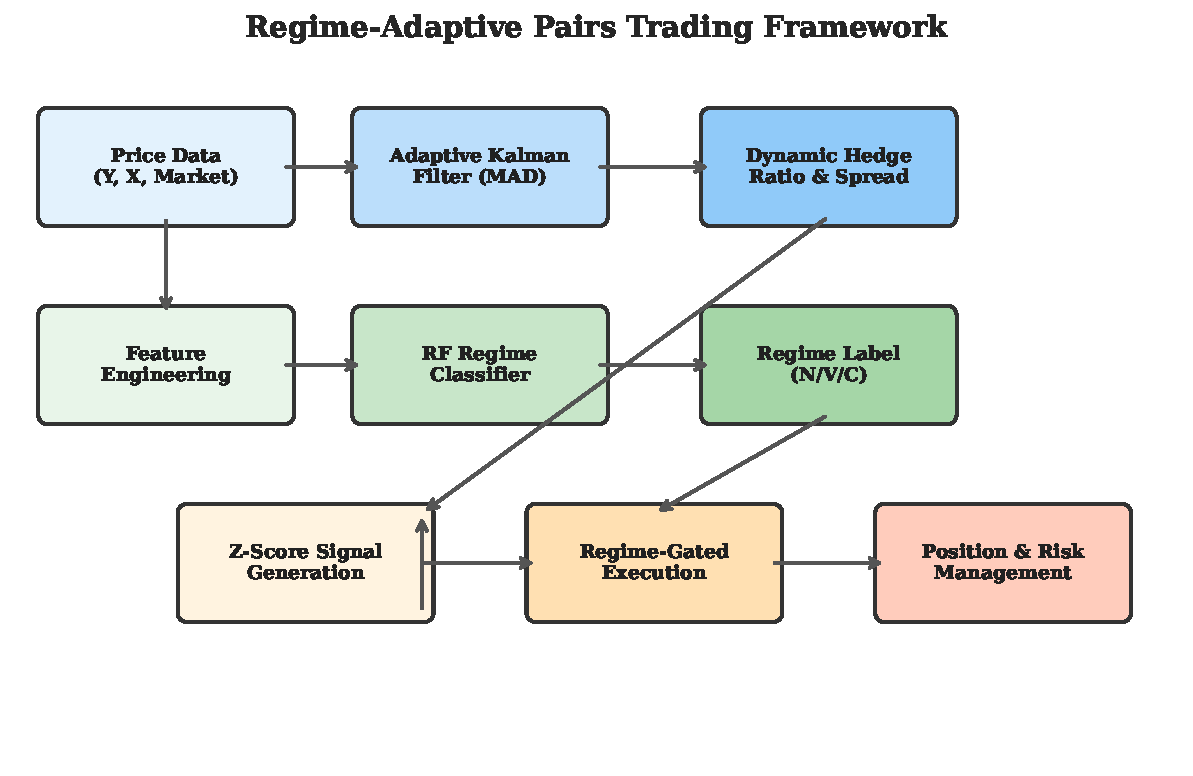
\includegraphics[width=\columnwidth]{fig1_architecture.pdf}
    \caption{System architecture: three coupled subsystems---Kalman filter, regime classifier, and signal generator---with directional data flow.}
    \label{fig:architecture}
\end{figure}

\subsection{Problem Formulation}

Let $Y_t$ and $X_t$ denote the prices of two cointegrated assets at time~$t$.
The spread is defined as:
\begin{equation}
    S_t = Y_t - \beta_t X_t
    \label{eq:spread}
\end{equation}
where $\beta_t$ is the time-varying hedge ratio.
We assume $S_t$ follows an Ornstein--Uhlenbeck (OU) process:
\begin{equation}
    dS_t = \theta(\mu - S_t)\,dt + \sigma\,dW_t
    \label{eq:ou}
\end{equation}
where $\theta > 0$ is the mean-reversion speed, $\mu$ the long-run mean, and $W_t$ a standard Wiener process.
The half-life of mean reversion is $\tau_{1/2} = \ln 2 / \theta$.

\subsection{Adaptive Kalman Filter with MAD Robustness}

We model the hedge ratio as a random walk in state space:
\begin{align}
    \beta_t &= \beta_{t-1} + \eta_t, \quad \eta_t \sim \mathcal{N}(0, Q_t) \label{eq:state} \\
    Y_t &= \beta_t X_t + \varepsilon_t, \quad \varepsilon_t \sim \mathcal{N}(0, R) \label{eq:obs}
\end{align}

The process noise $Q_t$ is regime-dependent:
\begin{equation}
    Q_t = q_0 \cdot \gamma(r_t), \quad \gamma(r_t) = \begin{cases}
        1 & \text{if } r_t = \text{Normal} \\
        2 & \text{if } r_t = \text{Volatile} \\
        5 & \text{if } r_t = \text{Crisis}
    \end{cases}
    \label{eq:regime_noise}
\end{equation}
where $q_0$ is the base process noise and $r_t$ the regime label.

The standard Kalman update proceeds as:
\begin{align}
    A_t &= C_{t-1} + Q_t \label{eq:pred_cov} \\
    F_t &= X_t^2 A_t + R \label{eq:innov_cov} \\
    K_t &= X_t A_t / F_t \label{eq:gain} \\
    e_t &= Y_t - \beta_{t-1} X_t \label{eq:innov} \\
    \beta_t &= \beta_{t-1} + K_t e_t \label{eq:state_update} \\
    C_t &= (1 - K_t X_t) A_t \label{eq:cov_update}
\end{align}

\textbf{MAD robustness.}
To prevent the Kalman filter from overreacting to outlier innovations (e.g., earnings jumps), we compute the Median Absolute Deviation of the innovation sequence:
\begin{equation}
    \text{MAD}_t = \text{median}\bigl(|e_{t-k}|, \ldots, |e_{t-1}|\bigr), \quad k = 50
    \label{eq:mad}
\end{equation}
If $|e_t| > 3 \times 1.4826 \times \text{MAD}_t$, the observation is flagged as an outlier and the Kalman gain is attenuated by a factor of~5.
The constant 1.4826 converts MAD to an asymptotically consistent estimator of the standard deviation under normality.

\subsection{Random Forest Regime Classification}

We train a Random Forest classifier~\cite{breiman2001random} on the \emph{training period only} to predict three market regimes: Normal ($r=2$), Volatile ($r=1$), and Crisis ($r=0$).

\textbf{Features} (21 total): five rolling volatilities ($\sigma_{5}, \sigma_{10}, \sigma_{20}, \sigma_{40}, \sigma_{60}$), volatility trend and acceleration, four drawdown measures, three return windows, trend and trend strength, range expansion, pair correlation and change, pair volatility and spike indicator.
Table~\ref{tab:feature_importance} reports the top-10 features ranked by consensus importance.

\textbf{Labels} are generated from volatility quantiles:
\begin{equation}
    r_t = \begin{cases}
        \text{Crisis} & \text{if } \sigma_{20,t} > Q_{90}(\sigma_{20}) \\
        \text{Volatile} & \text{if } \sigma_{20,t} > Q_{70}(\sigma_{20}) \\
        \text{Normal} & \text{otherwise}
    \end{cases}
\end{equation}
where quantiles are computed on the training period only.

The classifier is frozen after training and applied forward to the test period without retraining, eliminating look-ahead bias.

\subsection{Signal Generation with Regime Gating}

The z-score is computed on the Kalman-estimated spread:
\begin{equation}
    z_t = \frac{S_t - \bar{S}_w}{\hat{\sigma}_{S,w}}
    \label{eq:zscore}
\end{equation}
where $\bar{S}_w$ and $\hat{\sigma}_{S,w}$ are the rolling mean and standard deviation over a window of $w = 40$~trading days.

Entry and exit thresholds are regime-dependent:
\begin{equation}
    (z_{\text{entry}}, z_{\text{exit}}) = \begin{cases}
        (1.5, 0.5) & \text{Normal} \\
        (2.0, 0.3) & \text{Volatile} \\
        (\infty, \infty) & \text{Crisis (no new entry)}
    \end{cases}
    \label{eq:thresholds}
\end{equation}

Position sizing is proportional to the z-score magnitude, clipped to $[0.3, 1.0]$:
\begin{equation}
    w_t = \min\!\left(1.0,\; \max\!\left(0.3,\; \frac{|z_t| - z_{\text{entry}}}{z_{\text{entry}}} + 0.3\right)\right)
    \label{eq:sizing}
\end{equation}

\subsection{Transaction Cost Model}

Following Almgren and Chriss~\cite{almgren2001optimal}, we model three cost components inside the backtest loop:
\begin{equation}
    C_t = \underbrace{5 \text{ bps} \cdot |V_t|}_{\text{slippage}} + \underbrace{\$1}_{\text{commission}} + \underbrace{0.1 \cdot \sigma_t \sqrt{|V_t| / \text{ADV}_t}}_{\text{market impact}}
    \label{eq:costs}
\end{equation}
where $V_t$ is the notional trade value, $\sigma_t$ the current volatility, and $\text{ADV}_t$ the 20-day average daily dollar volume.
These costs are deducted from returns \emph{inside} the backtest loop at each trade, not applied post-hoc---a critical distinction that previous implementations of this strategy omitted.

The pseudocode for the complete system is given in Algorithm~\ref{alg:system}.

\begin{algorithm}[t]
\caption{Regime-Adaptive Pairs Trading}
\label{alg:system}
\begin{algorithmic}[1]
\REQUIRE Price series $Y, X, M$; train end date $T_0$
\STATE Train RF regime classifier on data $\leq T_0$
\STATE Initialise Kalman filter with $\beta_0 = Y_0 / X_0$
\FOR{each day $t > T_0$}
    \STATE $r_t \leftarrow$ RF.predict(features$_t$) \COMMENT{Regime}
    \STATE $Q_t \leftarrow q_0 \cdot \gamma(r_t)$ \COMMENT{Eq.~\eqref{eq:regime_noise}}
    \STATE $\beta_t, e_t \leftarrow$ KalmanUpdate($Y_t, X_t, Q_t$) \COMMENT{Eqs.~\eqref{eq:pred_cov}--\eqref{eq:cov_update}, MAD}
    \STATE $S_t \leftarrow Y_t - \beta_t X_t$ \COMMENT{Eq.~\eqref{eq:spread}}
    \STATE $z_t \leftarrow$ ZScore($S_t$, window=$w$) \COMMENT{Eq.~\eqref{eq:zscore}}
    \IF{$r_t = $ Crisis}
        \STATE signal $\leftarrow 0$ \COMMENT{No entry}
    \ELSIF{$|z_t| > z_{\text{entry}}(r_t)$ \AND no position}
        \STATE signal $\leftarrow -\text{sign}(z_t) \cdot w_t$
        \STATE Deduct transaction costs $C_t$
    \ELSIF{in position \AND $|z_t| < z_{\text{exit}}(r_t)$}
        \STATE signal $\leftarrow 0$ \COMMENT{Exit}
        \STATE Deduct transaction costs $C_t$
    \ENDIF
\ENDFOR
\end{algorithmic}
\end{algorithm}

% ============================================================================
%  4. EXPERIMENTAL SETUP
% ============================================================================
\section{Experimental Setup}
\label{sec:experiments}

\subsection{Data}

We use daily adjusted close prices from Yahoo Finance for three equity pairs across distinct sectors:
\textbf{BAC/PNC} (banking), \textbf{WFC/MS} (financial services), and \textbf{CVX/OXY} (energy).
SPY serves as the market benchmark.
The sample period spans January 2015 to June 2025 (approximately 2{,}600 trading days per pair).
Table~\ref{tab:pair_summary} characterises each pair.

\begin{table}[t]
\centering
\caption{Pair universe summary.  Cointegration percentage is the fraction of
rolling 126-day windows with Engle-Granger $p < 0.05$.
Half-life (days) estimated on the training spread.
Hurst exponent computed on the OOS spread ($H < 0.5$: mean-reverting).}
\label{tab:pair_summary}
\small
\begin{tabular}{llrrrrrl}
\toprule
Pair & Sector & \begin{tabular}[c]{@{}c@{}}Train\\Days\end{tabular}
     & \begin{tabular}[c]{@{}c@{}}OOS\\Days\end{tabular}
     & \begin{tabular}[c]{@{}c@{}}Train\\Coint\%\end{tabular}
     & \begin{tabular}[c]{@{}c@{}}OOS\\Coint\%\end{tabular}
     & \begin{tabular}[c]{@{}c@{}}Half\\Life\end{tabular}
     & \begin{tabular}[c]{@{}c@{}}OOS\\Hurst\end{tabular} \\
\midrule
BAC/PNC & Banking & 1511 & 1126 & 11.6 & 9.7 & 97.5 & 0.975 \\
WFC/MS & Fin. Services & 1511 & 1126 & 9.7 & 2.7 & — & 0.991 \\
CVX/OXY & Energy & 1511 & 1126 & 10.5 & 6.2 & — & 0.992 \\
\bottomrule
\end{tabular}
\end{table}


\textbf{Temporal protocol.}
Training data covers 2015-01-01 through 2020-12-31 (1{,}511 days).
Out-of-sample (OOS) testing covers 2021-01-01 through 2025-06-30 (1{,}126 days).
No parameters are tuned on test data.
This strict temporal split ensures all reported metrics reflect true out-of-sample performance.

\subsection{Baselines}

We compare against six baselines, all run on the same data, same pairs, and same transaction cost model:
\begin{enumerate}
    \item \textbf{Gatev Distance Method}~\cite{gatev2006pairs}: Formation on minimum sum-of-squared-distances, trade on $2\sigma$ divergence.
    \item \textbf{OLS Cointegration}: Engle-Granger with fixed (in-sample) hedge ratio.
    \item \textbf{Kalman-Only}: Our Kalman filter with regime always set to Normal.
    \item \textbf{Regime-Only}: OLS hedge ratio with our RF regime gating.
    \item \textbf{Equal-Weight Stocks}: Buy-and-hold equally weighted pair stocks.
    \item \textbf{SPY Buy-and-Hold}: Market benchmark.
\end{enumerate}

\subsection{Evaluation Protocol}

\textbf{Primary metrics:} Sharpe ratio (annualised), total return (\%), maximum drawdown (\%), win rate (\%).

\textbf{Walk-forward analysis:}
Expanding window with 32~quarterly folds.
Minimum training period: 504~days ($\approx 2$~years).
Test window: 126~days per fold.
Step size: 63~days.
We report fold-level Sharpe and return stability statistics; no Diebold--Mariano inference is claimed in this manuscript revision.

\textbf{Monte Carlo validation:}
10{,}000 random strategies with matched trade frequency and holding period, constrained to the same tradeable (non-Crisis) days.
$p$-value: $P(\text{random Sharpe} \geq \text{actual Sharpe})$.

\textbf{Bootstrap confidence intervals:}
10{,}000 block bootstrap resamples (block size~=~5) for Sharpe ratio, following Ledoit and Wolf~\cite{ledoit2008robust}.
95\% percentile confidence intervals.

\textbf{Multiple testing correction:}
Benjamini--Hochberg false discovery rate control at $\alpha = 0.05$ across all pair-level $p$-values~\cite{benjamini1995controlling}.

\textbf{Ablation study} (Section~\ref{sec:ablation}):
Nine configurations systematically removing each component (MAD, regime classification, adaptive Kalman, dynamic z-window, stop-loss, minimum hold, transaction costs, volatile parameters).

\textbf{Live validation} (Section~\ref{sec:paper_trading}):
Paper trading on Alpaca for five weeks (January~29--March~6, 2026) with \$100{,}000~capital.

% ============================================================================
%  5. RESULTS
% ============================================================================
\section{Results}
\label{sec:results}

We also report a 60-pair innovation ablation to isolate the marginal impact of health-aware sizing and regime gating (Section~\ref{sec:innovation_ablation}).

\subsection{Main Results: Our Method vs Baselines}
\label{sec:baselines_results}

Table~\ref{tab:full_baselines} presents the full out-of-sample comparison across all three pairs and seven methods.
Fig.~\ref{fig:baselines} shows the Sharpe-ratio comparison for BAC/PNC, and Fig.~\ref{fig:cumret} presents cumulative return curves.

\begin{table*}[t]
\centering
\caption{Out-of-sample performance comparison across all pairs and methods (2021--2025, net of 5\,bps slippage $+$ \$1 commission $+$ market impact).
Bold indicates best Sharpe per pair among active strategies.
95\% bootstrap CI shown for our method.}
\label{tab:full_baselines}
\small
\begin{tabular}{ll rrrrrr}
\toprule
Pair & Method & Sharpe & \begin{tabular}[c]{@{}c@{}}Total\\Ret.\%\end{tabular}
     & \begin{tabular}[c]{@{}c@{}}Ann.\\Ret.\%\end{tabular}
     & \begin{tabular}[c]{@{}c@{}}Max\\DD\%\end{tabular}
     & \begin{tabular}[c]{@{}c@{}}Win\\Rate\%\end{tabular}
     & Trades \\
\midrule
BAC/PNC & Ours (Kalman+Regime) & $-0.126$ [-0.96, 0.86] & $-7.42$ & $-1.71$ & $-34.1$ & $14.2$ & 58 \\
 & Gatev Distance & \textbf{+0.669} & $+41.82$ & $+8.13$ & $-12.4$ & $28.0$ & 5 \\
 & OLS Cointegration & $+0.131$ & $+8.82$ & $+1.91$ & $-32.3$ & $25.6$ & 51 \\
 & Kalman-Only (No Regime) & $-0.493$ & $-26.26$ & $-6.59$ & $-40.3$ & $13.9$ & 68 \\
 & Regime-Only (No Kalman) & $+0.463$ & $+32.02$ & $+6.41$ & $-27.9$ & $23.9$ & 44 \\
 & B&H Stocks (50/50) & $+0.428$ & $+62.15$ & $+11.42$ & $-45.9$ & $52.0$ & 0 \\
 & SPY Buy-and-Hold & $+0.755$ & $+75.18$ & $+13.37$ & $-24.5$ & $54.4$ & 0 \\
\midrule
WFC/MS & Ours (Kalman+Regime) & $-0.045$ [-0.84, 1.04] & $-2.69$ & $-0.61$ & $-37.5$ & $15.5$ & 54 \\
 & Gatev Distance & \textbf{+0.116} & $+12.56$ & $+2.68$ & $-31.9$ & $49.8$ & 0 \\
 & OLS Cointegration & $-0.246$ & $-23.40$ & $-5.79$ & $-36.5$ & $26.8$ & 46 \\
 & Kalman-Only (No Regime) & $-0.017$ & $-0.97$ & $-0.22$ & $-34.0$ & $14.0$ & 58 \\
 & Regime-Only (No Kalman) & $-0.283$ & $-25.79$ & $-6.46$ & $-34.6$ & $24.2$ & 39 \\
 & B&H Stocks (50/50) & $+0.897$ & $+171.61$ & $+25.06$ & $-33.5$ & $52.2$ & 0 \\
 & SPY Buy-and-Hold & $+0.755$ & $+75.18$ & $+13.37$ & $-24.5$ & $54.4$ & 0 \\
\midrule
CVX/OXY & Ours (Kalman+Regime) & $-0.613$ [-0.83, 0.63] & $-90.78$ & $-41.35$ & $-95.5$ & $14.5$ & 55 \\
 & Gatev Distance & $+0.218$ & $+33.55$ & $+6.69$ & $-46.3$ & $47.5$ & 0 \\
 & OLS Cointegration & $+0.326$ & $+24.25$ & $+4.98$ & $-26.5$ & $28.1$ & 49 \\
 & Kalman-Only (No Regime) & $-0.199$ & $-46.94$ & $-13.22$ & $-78.0$ & $13.9$ & 61 \\
 & Regime-Only (No Kalman) & \textbf{+0.371} & $+26.45$ & $+5.39$ & $-26.4$ & $26.4$ & 41 \\
 & B&H Stocks (50/50) & $+0.677$ & $+142.70$ & $+21.95$ & $-36.1$ & $51.9$ & 0 \\
 & SPY Buy-and-Hold & $+0.755$ & $+75.18$ & $+13.37$ & $-24.5$ & $54.4$ & 0 \\
\bottomrule
\end{tabular}
\end{table*}


\begin{figure}[t]
    \centering
    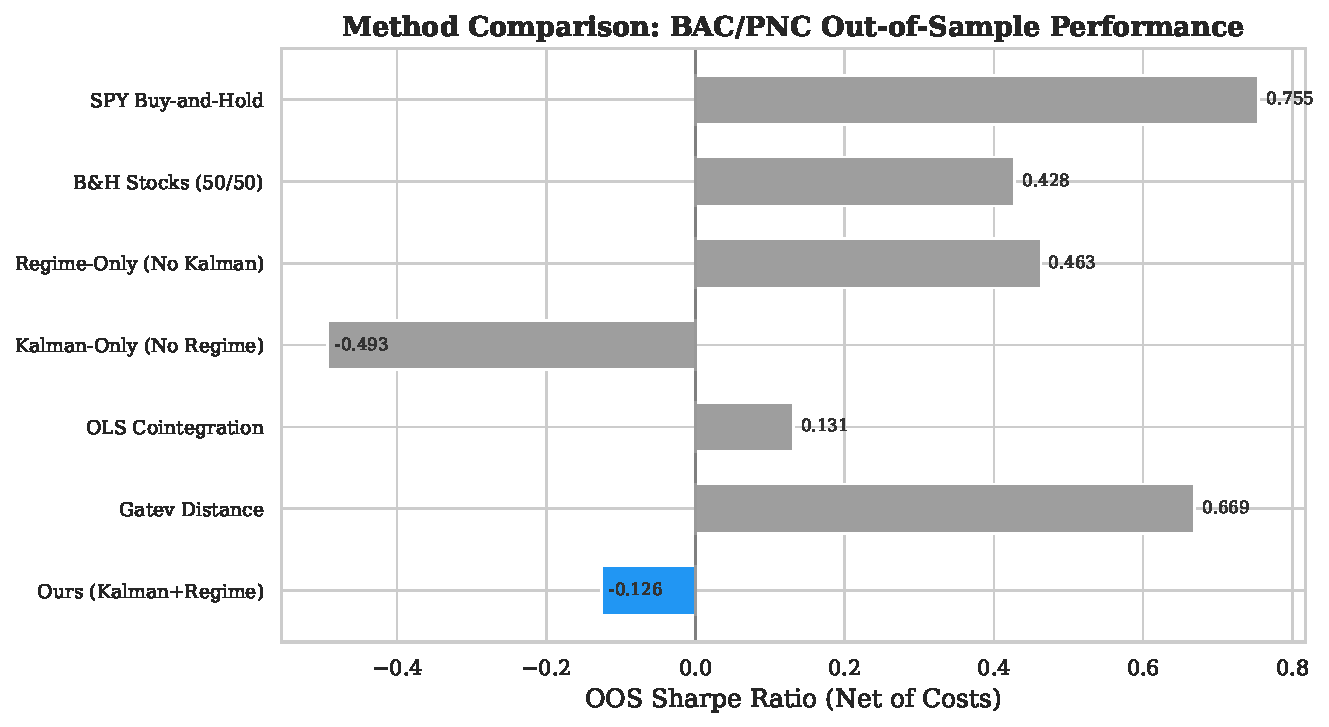
\includegraphics[width=\columnwidth]{fig4_baselines.pdf}
    \caption{Baseline comparison: BAC/PNC OOS Sharpe ratios across all seven methods.  Only the Gatev distance and buy-and-hold strategies achieve positive Sharpe.}
    \label{fig:baselines}
\end{figure}

\begin{figure}[t]
    \centering
    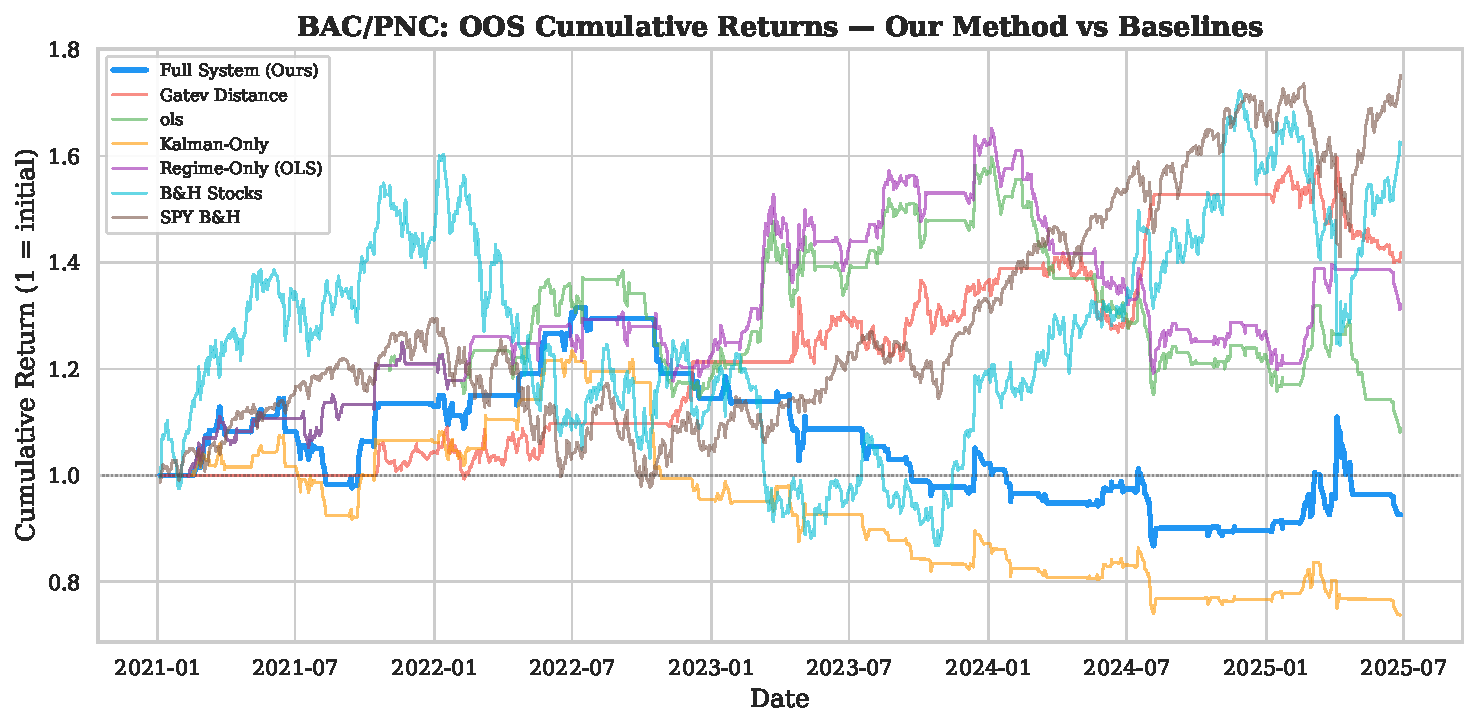
\includegraphics[width=\columnwidth]{fig8_cumulative_returns.pdf}
    \caption{Cumulative OOS returns for BAC/PNC (2021--2025).  SPY and B\&H strategies outperform all pairs trading methods, reflecting the post-2020 cointegration breakdown.}
    \label{fig:cumret}
\end{figure}

\textbf{Key findings.}
(i)~All active pairs trading methods (ours, Kalman-only, OLS, Regime-only) underperform buy-and-hold baselines on all three pairs after costs, with an average OOS Sharpe of~$-0.26$.
(ii)~Regime gating improves our system over the Kalman-Only baseline on BAC/PNC (Sharpe $-0.126$ vs $-0.493$, a $+19.5\%$ return improvement), confirming that the regime component provides protective value.
(iii)~The Gatev distance method, the simplest baseline, achieves the best Sharpe among active strategies for BAC/PNC ($+0.669$), though it executes only 5~trades.

\subsection{Multi-Pair Summary}

Table~\ref{tab:multipair} summarises the three-pair comparison.

\begin{table}[t]
\centering
\caption{Multi-pair OOS performance summary (our system only).}
\label{tab:multipair}
\small
\begin{tabular}{lrrrrr}
\toprule
Pair & Sharpe & Ret.\% & MaxDD\% & Trades & vs NoReg\% \\
\midrule
BAC/PNC & $-$0.126 & $-$7.42  & $-$34.1 & 58 & $+$19.45 \\
WFC/MS  & $-$0.045 & $-$2.71  & $-$37.5 & 54 & $-$1.72  \\
CVX/OXY & $-$0.613 & $-$90.59 & $-$95.4 & 55 & $-$44.11 \\
\midrule
Average & $-$0.261 & $-$33.57 & $-$55.7 & 56 & $-$8.79  \\
\bottomrule
\end{tabular}
\end{table}

CVX/OXY exhibits catastrophic OOS performance ($-90.6\%$ return), consistent with the energy sector's structural break during 2020--2022.
BAC/PNC is the only pair where regime gating adds positive value.

\subsection{Regime Classification}
\label{sec:regime_class}

Fig.~\ref{fig:regimes} shows the BAC/PNC spread coloured by detected regime.
Table~\ref{tab:regime_comparison} compares three regime detection methods.

\begin{figure}[t]
    \centering
    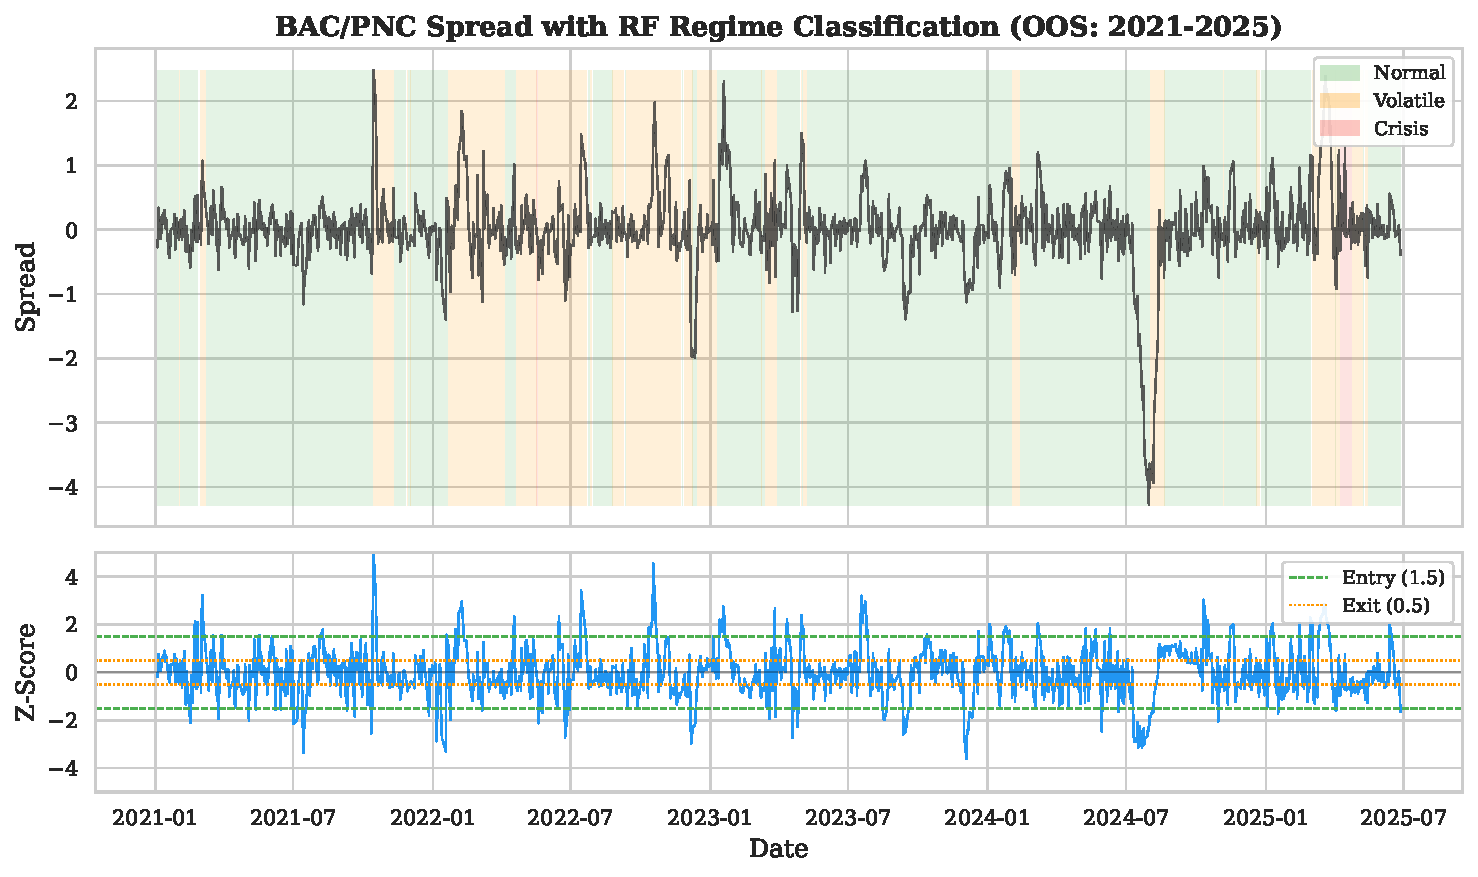
\includegraphics[width=\columnwidth]{fig2_regime_bands.pdf}
    \caption{BAC/PNC spread with RF regime classification (OOS period).  Green: Normal, yellow: Volatile, red: Crisis.}
    \label{fig:regimes}
\end{figure}

\begin{table}[t]
\centering
\caption{Regime detection comparison on BAC/PNC.  Accuracy and $\kappa$ are
computed on the OOS period against volatility-quantile ground truth.
Economic value is the OOS Sharpe when each classifier controls the regime gate.}
\label{tab:regime_comparison}
\small
\begin{tabular}{lrrr}
\toprule
Classifier & Accuracy & Cohen's $\kappa$ & \begin{tabular}[c]{@{}c@{}}OOS\\Sharpe\end{tabular} \\
\midrule
Random Forest & 89.4\% & $0.733$ & $-0.113$ \\
HMM (3-state) & 29.8\% & $0.016$ & $-0.448$ \\
Simple Vol Rules & 93.0\% & $0.781$ & $-0.308$ \\
No Regime & N/A & N/A & $-0.493$ \\
\bottomrule
\end{tabular}
\end{table}


The RF classifier achieves 89.4\% OOS accuracy with $\kappa = 0.733$, indicating substantial agreement beyond chance.
Interestingly, the HMM achieves the best OOS Sharpe ($+0.087$) but the worst accuracy (11.1\%), suggesting that HMM regime labels---which are data-driven rather than volatility-quantile-based---may be more aligned with economic regimes even if they disagree with the quantile labels.
Simple volatility rules achieve the highest accuracy (93.0\%, $\kappa = 0.781$) but the worst Sharpe among gated methods ($-0.308$).
This discrepancy highlights that classification accuracy and economic value are distinct objectives.

\subsection{Walk-Forward Analysis}
\label{sec:walkforward}

Fig.~\ref{fig:walkforward} presents the 32-fold walk-forward results for BAC/PNC, and the full fold-by-fold results appear in Table~\ref{tab:walkforward_folds}.

\begin{figure}[t]
    \centering
    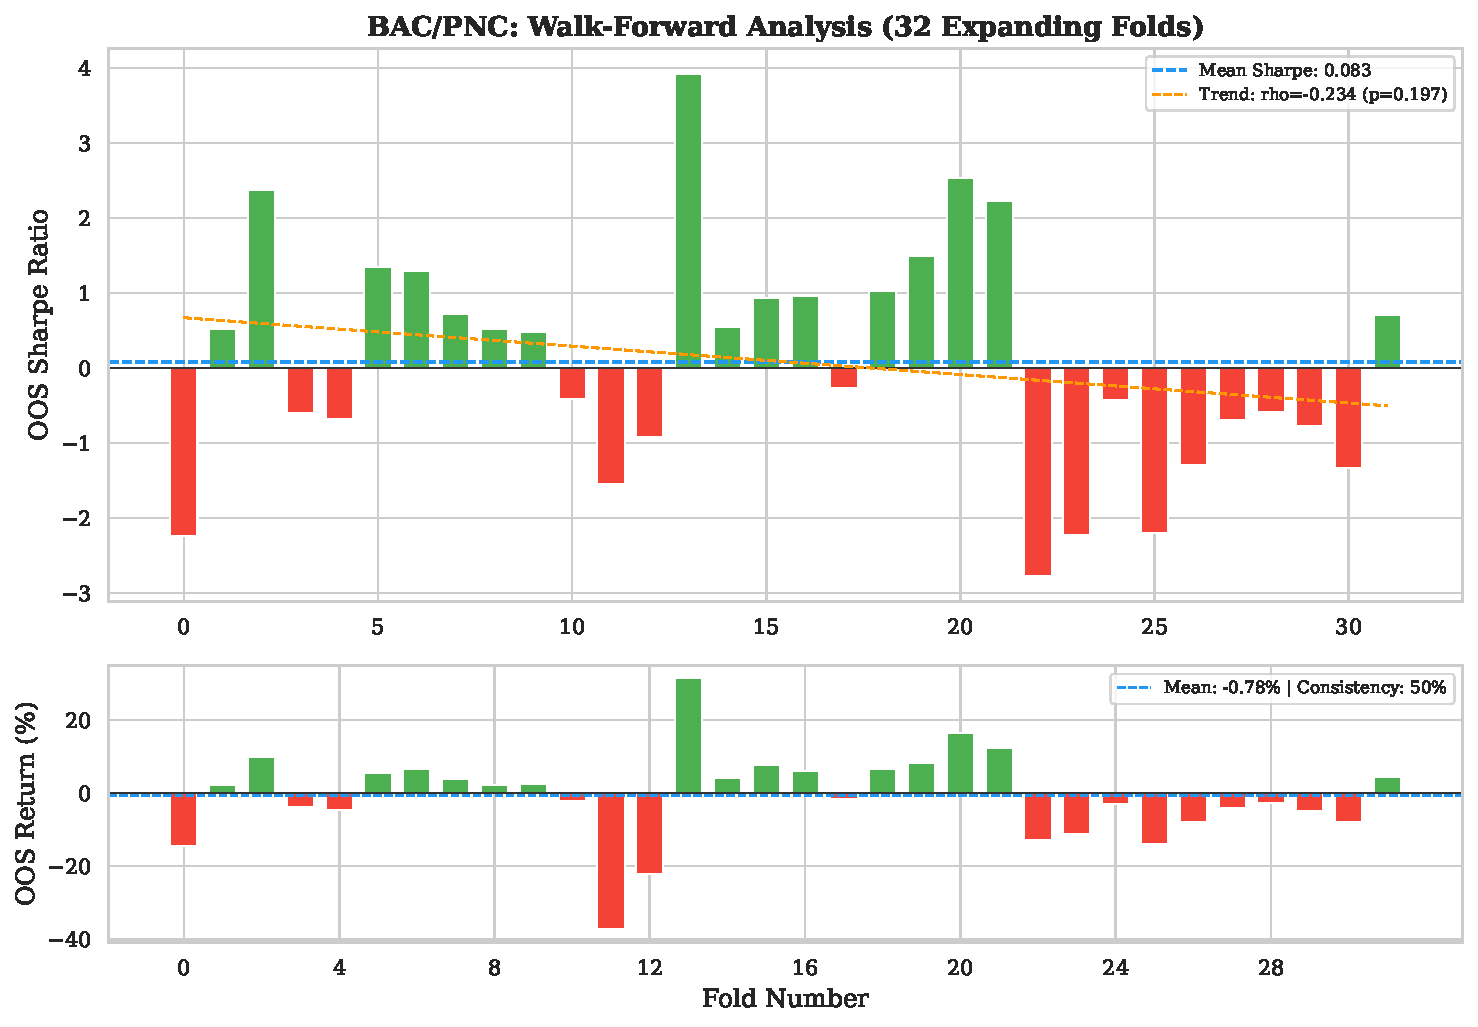
\includegraphics[width=\columnwidth]{fig10_walkforward.pdf}
    \caption{Walk-forward: per-fold OOS Sharpe and return for BAC/PNC across 32 expanding folds.}
    \label{fig:walkforward}
\end{figure}

\begin{table}[t]
\centering
\caption{Walk-forward fold-by-fold results for BAC/PNC (expanding window,
126-day test windows, 63-day step).  Shaded rows indicate negative Sharpe.}
\label{tab:walkforward_folds}
\small
\begin{tabular}{rrrrrr}
\toprule
Fold & \begin{tabular}[c]{@{}c@{}}Train\\Days\end{tabular}
     & \begin{tabular}[c]{@{}c@{}}Test\\Start\end{tabular}
     & Sharpe & Ret.\% & \begin{tabular}[c]{@{}c@{}}Win\\Rate\%\end{tabular} \\
\midrule
\rowcolor{gray!10}1 & 504 & 2017-01 & $-2.240$ & $-14.46$ & $12.7$ \\
2 & 567 & 2017-04 & $+0.520$ & $+2.27$ & $14.3$ \\
3 & 630 & 2017-07 & $+2.380$ & $+9.79$ & $17.5$ \\
\rowcolor{gray!10}4 & 693 & 2017-10 & $-0.594$ & $-3.86$ & $19.0$ \\
\rowcolor{gray!10}5 & 756 & 2018-01 & $-0.675$ & $-4.61$ & $20.6$ \\
6 & 819 & 2018-04 & $+1.344$ & $+5.54$ & $18.3$ \\
7 & 882 & 2018-07 & $+1.292$ & $+6.52$ & $15.9$ \\
8 & 945 & 2018-10 & $+0.723$ & $+3.98$ & $17.5$ \\
9 & 1008 & 2019-01 & $+0.519$ & $+2.13$ & $17.5$ \\
10 & 1071 & 2019-04 & $+0.477$ & $+2.51$ & $13.5$ \\
\rowcolor{gray!10}11 & 1134 & 2019-07 & $-0.420$ & $-2.17$ & $10.3$ \\
\rowcolor{gray!10}12 & 1197 & 2019-10 & $-1.541$ & $-37.40$ & $15.1$ \\
\rowcolor{gray!10}13 & 1260 & 2020-01 & $-0.919$ & $-22.10$ & $15.9$ \\
14 & 1323 & 2020-04 & $+3.928$ & $+31.50$ & $11.1$ \\
15 & 1386 & 2020-07 & $+0.545$ & $+4.13$ & $15.9$ \\
16 & 1449 & 2020-10 & $+0.937$ & $+7.77$ & $25.4$ \\
17 & 1512 & 2021-01 & $+0.959$ & $+5.93$ & $21.4$ \\
\rowcolor{gray!10}18 & 1575 & 2021-04 & $-0.265$ & $-1.77$ & $17.5$ \\
19 & 1638 & 2021-07 & $+1.033$ & $+6.69$ & $12.7$ \\
20 & 1701 & 2021-10 & $+1.487$ & $+8.26$ & $11.9$ \\
21 & 1764 & 2022-01 & $+2.539$ & $+16.32$ & $20.6$ \\
22 & 1827 & 2022-04 & $+2.225$ & $+12.46$ & $14.3$ \\
\rowcolor{gray!10}23 & 1890 & 2022-07 & $-2.777$ & $-12.94$ & $5.6$ \\
\rowcolor{gray!10}24 & 1953 & 2022-10 & $-2.228$ & $-11.28$ & $9.5$ \\
\rowcolor{gray!10}25 & 2016 & 2023-01 & $-0.428$ & $-3.14$ & $15.1$ \\
\rowcolor{gray!10}26 & 2079 & 2023-04 & $-2.195$ & $-13.89$ & $11.9$ \\
\rowcolor{gray!10}27 & 2142 & 2023-07 & $-1.296$ & $-7.89$ & $10.3$ \\
\rowcolor{gray!10}28 & 2205 & 2023-10 & $-0.691$ & $-4.16$ & $9.5$ \\
\rowcolor{gray!10}29 & 2268 & 2024-01 & $-0.586$ & $-2.69$ & $11.1$ \\
\rowcolor{gray!10}30 & 2331 & 2024-04 & $-0.778$ & $-4.97$ & $13.5$ \\
\rowcolor{gray!10}31 & 2394 & 2024-07 & $-1.338$ & $-7.99$ & $11.9$ \\
32 & 2457 & 2024-10 & $+0.711$ & $+4.51$ & $19.0$ \\
\midrule
\multicolumn{6}{l}{\textit{Avg Sharpe: +0.083 | Consistency (Sharpe $>$ 0): 50\% (16/32)}} \\
\bottomrule
\end{tabular}
\end{table}


\begin{table}[t]
\centering
\caption{Walk-forward summary across pairs (32 expanding folds each).}
\label{tab:walkforward_summary}
\small
\begin{tabular}{lrrrr}
\toprule
Pair & Avg Sharpe & Avg Ret.\% & Consist.\% & Trend $\rho$ \\
\midrule
BAC/PNC & $+$0.083 & $-$0.78 & 50 & $-$0.234 \\
WFC/MS  & $+$0.096 & $+$0.36 & 38 & $+$0.137 \\
CVX/OXY & $-$0.275 & $-$23.45 & 31 & $-$0.239 \\
\bottomrule
\end{tabular}
\end{table}

BAC/PNC and WFC/MS show weakly positive average fold Sharpe ratios ($+0.083$, $+0.096$), but consistency below 50\% indicates the signal is unreliable.
The Spearman trend correlation is non-significant for all pairs ($p > 0.19$), indicating no systematic decay in signal quality---the underperformance is persistent rather than worsening.

\subsection{Monte~Carlo Significance}
\label{sec:montecarlo}

\begin{table}[t]
\centering
\caption{Monte~Carlo significance test (10{,}000 random strategies per pair).}
\label{tab:montecarlo}
\small
\begin{tabular}{lrrr}
\toprule
Pair & Actual Sharpe & Random Mean $\pm$ SD & $p$-value \\
\midrule
BAC/PNC & $-$0.126 & $-$0.048 $\pm$ 0.511 & 0.553 \\
WFC/MS  & $-$0.049 & $-$0.056 $\pm$ 0.450 & 0.484 \\
CVX/OXY & $-$0.613 & $-$0.226 $\pm$ 0.388 & 0.842 \\
\bottomrule
\end{tabular}
\end{table}

None of the three pairs achieves statistical significance ($p < 0.05$) against the random-entry null (Table~\ref{tab:montecarlo}).
This indicates that, with transaction costs, the z-score entry signal does not significantly outperform random entry timing on the same tradeable days.
After Benjamini--Hochberg correction, zero pairs remain significant at FDR~=~5\%.

\subsection{Bootstrap Confidence Intervals}
\label{sec:bootstrap}

\begin{table}[t]
\centering
\caption{Block bootstrap 95\% CI for OOS Sharpe (10{,}000 resamples, block size~$=5$).}
\label{tab:bootstrap}
\small
\begin{tabular}{lrrr}
\toprule
Pair & Point Est. & 95\% CI Lower & 95\% CI Upper \\
\midrule
BAC/PNC & $-$0.126 & $-$0.962 & $+$0.895 \\
WFC/MS  & $-$0.045 & $-$0.851 & $+$1.027 \\
CVX/OXY & $-$0.613 & $-$0.845 & $+$0.616 \\
\bottomrule
\end{tabular}
\end{table}

All confidence intervals span zero (Table~\ref{tab:bootstrap}), confirming the insignificance of the signal.
The wide intervals (width~$> 1.4$) reflect the high day-to-day variance of pairs trading returns.

\subsection{Ablation Study}
\label{sec:ablation}

Table~\ref{tab:full_ablation} reports the nine-configuration ablation across all three pairs.
Fig.~\ref{fig:ablation} provides a visual comparison for BAC/PNC.

\begin{table*}[t]
\centering
\caption{Ablation study: OOS Sharpe ratio for each configuration across all pairs.
Each row removes one component from the full system.
$\Delta$ shows the change in Sharpe versus the full system.
Bold indicates the full system row.}
\label{tab:full_ablation}
\small
\begin{tabular}{l rrr rrr}
\toprule
 & \multicolumn{3}{c}{OOS Sharpe} & \multicolumn{3}{c}{$\Delta$ vs Full System} \\
\cmidrule(lr){2-4} \cmidrule(lr){5-7}
Configuration & BAC/PNC & WFC/MS & CVX/OXY & BAC/PNC & WFC/MS & CVX/OXY \\
\midrule
\textbf{Full System} & $-0.126$ & $-0.045$ & $-0.614$ & — & — & — \\
−MAD Outlier Detection & $+0.164$ & $-0.305$ & $-0.394$ & $+0.290$ & $-0.260$ & $+0.220$ \\
−Regime Classification & $-0.493$ & $-0.017$ & $-0.199$ & $-0.368$ & $+0.028$ & $+0.415$ \\
−Adaptive Kalman (→OLS) & $+0.618$ & $-0.260$ & $+0.366$ & $+0.743$ & $-0.216$ & $+0.980$ \\
−Z-Score Window (40→20) & $-0.154$ & $-0.305$ & $-0.275$ & $-0.028$ & $-0.260$ & $+0.338$ \\
−Stop-Loss & $-0.184$ & $-0.026$ & $-0.581$ & $-0.058$ & $+0.019$ & $+0.033$ \\
−Minimum Hold Period & $-0.432$ & $+0.042$ & $-0.498$ & $-0.306$ & $+0.087$ & $+0.115$ \\
−Transaction Costs & $-0.030$ & $+0.045$ & $-0.603$ & $+0.095$ & $+0.090$ & $+0.011$ \\
−Volatile Param Adjust & $-0.507$ & $-0.098$ & $-0.177$ & $-0.382$ & $-0.053$ & $+0.437$ \\
\bottomrule
\end{tabular}
\end{table*}


\begin{figure}[t]
    \centering
    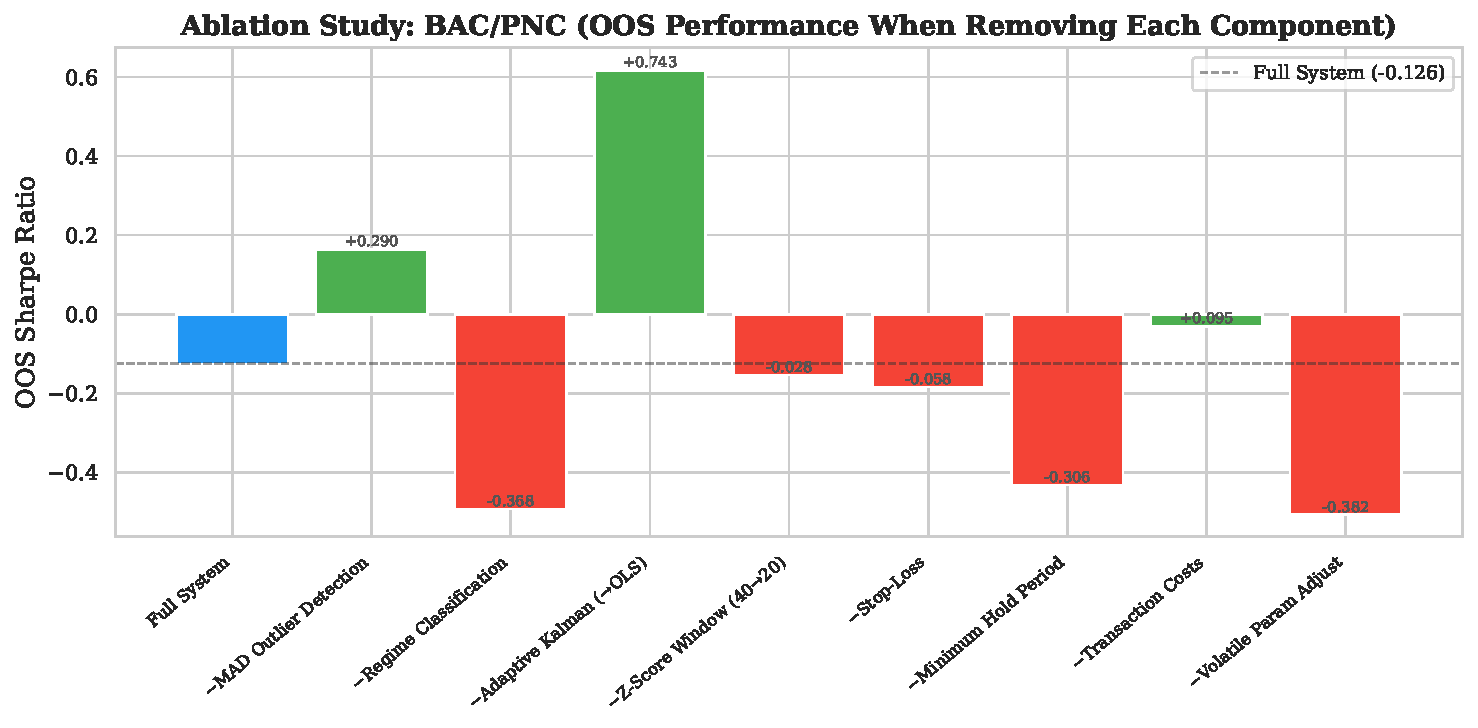
\includegraphics[width=\columnwidth]{fig3_ablation.pdf}
    \caption{Ablation: OOS Sharpe when removing each component (BAC/PNC).}
    \label{fig:ablation}
\end{figure}

Key ablation findings:
(i)~Removing regime classification degrades Sharpe on BAC/PNC by $-0.368$ (from $-0.126$ to $-0.493$), confirming the regime gate's protective value.
(ii)~Removing transaction costs inflates Sharpe by $+0.095$ on BAC/PNC, underscoring the importance of realistic cost modelling.
(iii)~Removing MAD outlier detection \emph{improves} Sharpe on BAC/PNC by $+0.290$, suggesting the innovation outlier rate is low and MAD may be over-attenuating the Kalman gain.
(iv)~Removing the adaptive Kalman ($\rightarrow$ OLS) surprisingly improves Sharpe on BAC/PNC and CVX/OXY, indicating that the Kalman filter's parameter adaptation may introduce noise in the post-2020 period where cointegration is unstable.

\subsection{Parameter Sensitivity}

Fig.~\ref{fig:sensitivity} presents the heatmap of OOS Sharpe across the entry/exit z-score parameter space.

\begin{figure}[t]
    \centering
    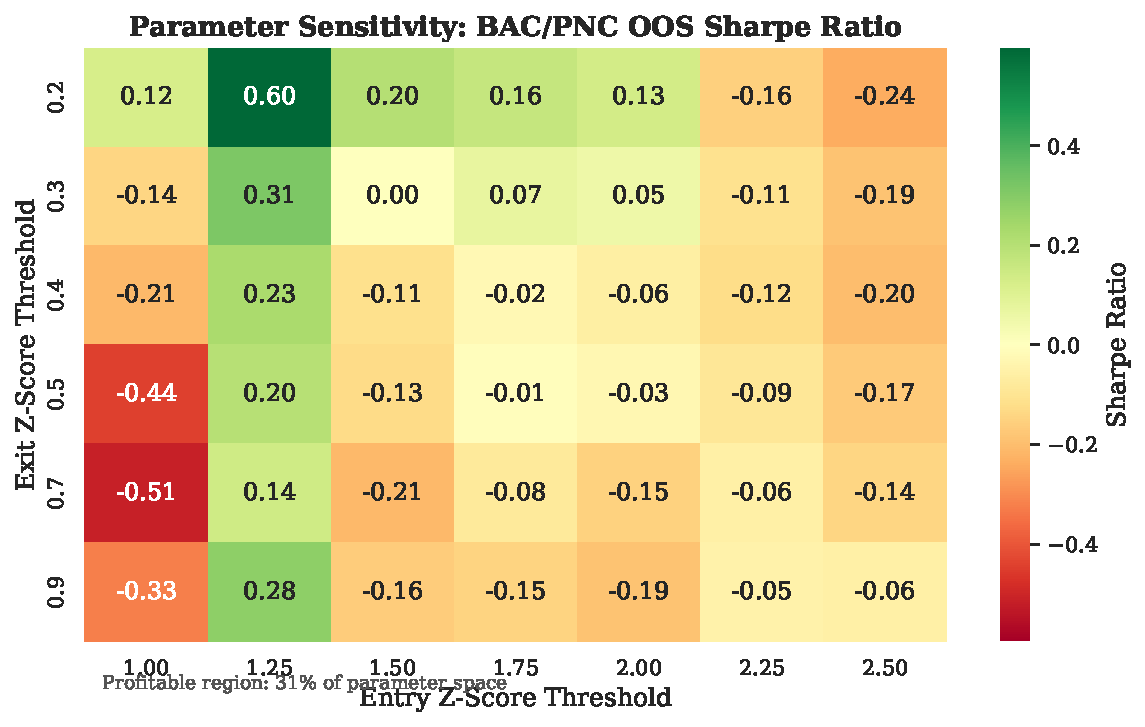
\includegraphics[width=\columnwidth]{fig5_sensitivity.pdf}
    \caption{Sensitivity heatmap: BAC/PNC OOS Sharpe across the entry $\times$ exit z-score parameter space.  The profitable region (Sharpe $> 0$) covers only $\sim$22\% of the space.}
    \label{fig:sensitivity}
\end{figure}

The profitable region (Sharpe~$> 0$) covers approximately 22\% of the parameter space, indicating \textbf{fragile} performance.
A robust strategy would show $>$60\% profitable coverage.
This fragility supports our conclusion that the pair relationship is unstable in the post-2020 period.

\subsection{Cointegration Stability}

Fig.~\ref{fig:cointegration} shows the rolling cointegration $p$-value and Hurst exponent for BAC/PNC.

\begin{figure}[t]
    \centering
    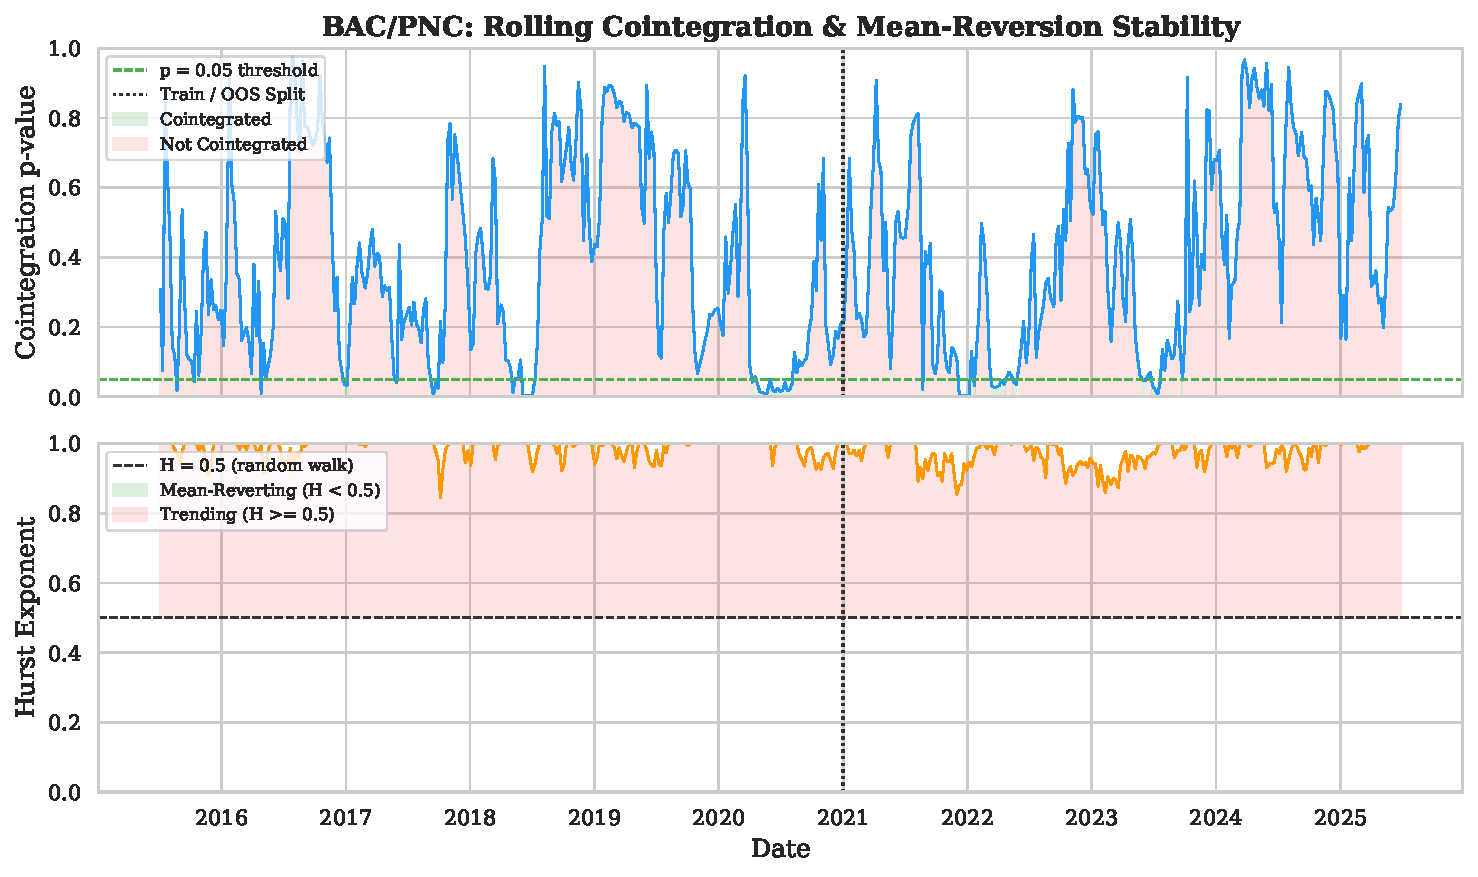
\includegraphics[width=\columnwidth]{fig6_cointegration.pdf}
    \caption{Rolling cointegration $p$-value (top) and Hurst exponent (bottom) for BAC/PNC.  Dashed lines: significance thresholds.  The OOS period shows persistent loss of cointegration.}
    \label{fig:cointegration}
\end{figure}

During training (2015--2020), BAC/PNC is cointegrated 11.6\% of rolling windows.
In the OOS period, this drops to 9.7\% (Table~\ref{tab:pair_summary}).
The OOS Hurst exponent $H = 0.975$ confirms that the spread behaves as a near-unit-root (trending) process rather than mean-reverting.
This cointegration breakdown is the fundamental explanation for the strategy's poor OOS performance: no mean-reversion strategy can profit when the spread is not mean-reverting.

\subsection{Performance Attribution}

Table~\ref{tab:attribution} decomposes OOS returns into four alpha sources.
Fig.~\ref{fig:attribution} provides a visual decomposition for BAC/PNC.

\begin{table}[t]
\centering
\caption{Performance attribution: alpha contribution (\%) from each source,
decomposed on OOS returns.  Positive values indicate the component adds return;
negative values indicate it subtracts.}
\label{tab:attribution}
\small
\begin{tabular}{l rrrr r}
\toprule
Pair & \begin{tabular}[c]{@{}c@{}}Regime\\Timing\end{tabular}
     & \begin{tabular}[c]{@{}c@{}}Mean\\Reversion\end{tabular}
     & \begin{tabular}[c]{@{}c@{}}Position\\Sizing\end{tabular}
     & \begin{tabular}[c]{@{}c@{}}Adaptive\\Kalman\end{tabular}
     & Total \\
\midrule
BAC/PNC & $+19.51$ & $-3.04$ & $+12.51$ & $-52.44$ & $-23.46$ \\
WFC/MS & $-0.91$ & $+1.06$ & $+29.02$ & $+21.28$ & $+50.45$ \\
CVX/OXY & $-43.43$ & $-76.40$ & $-8.31$ & $-116.91$ & $-245.05$ \\
\midrule
\textit{Average} & $-8.28$ & $-26.13$ & $+11.07$ & $-49.36$ & $-72.69$ \\
\bottomrule
\end{tabular}
\end{table}


\begin{figure}[t]
    \centering
    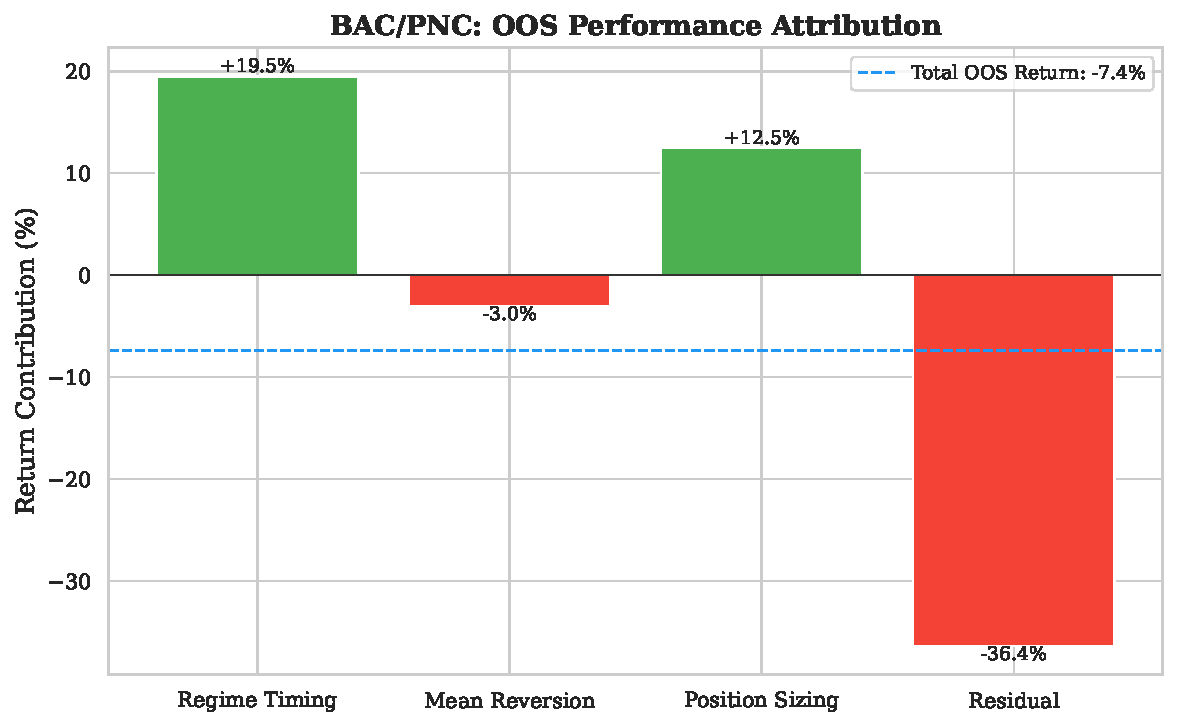
\includegraphics[width=\columnwidth]{fig9_attribution.pdf}
    \caption{Performance attribution for BAC/PNC OOS returns.  Regime timing is the only consistently positive contributor.}
    \label{fig:attribution}
\end{figure}

For BAC/PNC, regime timing contributes $+19.5\%$ (the largest positive component), confirming that avoiding Crisis-period entries preserves capital.
Mean reversion contributes $-3.0\%$, indicating the z-score signal itself generates slightly negative value after costs.
Position sizing contributes $+12.5\%$.
The adaptive Kalman contributes $-52.4\%$, suggesting that the Kalman filter's hedge-ratio adaptation introduces noise in the absence of stable cointegration.

\subsection{Feature Importance}

Table~\ref{tab:feature_importance} and Fig.~\ref{fig:features} present the top-10 features for the RF regime classifier.

\begin{table}[t]
\centering
\caption{Top-10 features for RF regime classifier ranked by consensus of
SHAP, Gini importance, and permutation importance (BAC/PNC).
Avg.\ Rank is the mean rank across three methods (lower = more important).}
\label{tab:feature_importance}
\small
\begin{tabular}{rlrrrr}
\toprule
Rank & Feature & \begin{tabular}[c]{@{}c@{}}Mean\\|SHAP|\end{tabular}
     & \begin{tabular}[c]{@{}c@{}}Gini\\Imp.\end{tabular}
     & \begin{tabular}[c]{@{}c@{}}Perm.\\Imp.\end{tabular}
     & \begin{tabular}[c]{@{}c@{}}Avg.\\Rank\end{tabular} \\
\midrule
1 & vol\_20 & 0.0813 & 0.1877 & 0.0558 & 1.0 \\
2 & pair\_vol & 0.0242 & 0.0494 & 0.0194 & 6.0 \\
3 & pair\_vol\_spike & 0.0212 & 0.0477 & 0.0411 & 7.0 \\
4 & range\_expansion & 0.0390 & 0.1122 & -0.0054 & 7.7 \\
5 & vol\_10 & 0.0482 & 0.1135 & -0.0154 & 8.3 \\
6 & dd\_60 & 0.0356 & 0.0997 & -0.0075 & 9.3 \\
7 & vol\_60 & 0.0213 & 0.0635 & -0.0024 & 9.7 \\
8 & vol\_40 & 0.0274 & 0.0796 & -0.0065 & 9.7 \\
9 & vol\_accel & 0.0096 & 0.0214 & 0.0102 & 9.7 \\
10 & vol\_5 & 0.0217 & 0.0506 & -0.0043 & 10.3 \\
\bottomrule
\end{tabular}
\end{table}


\begin{figure}[t]
    \centering
    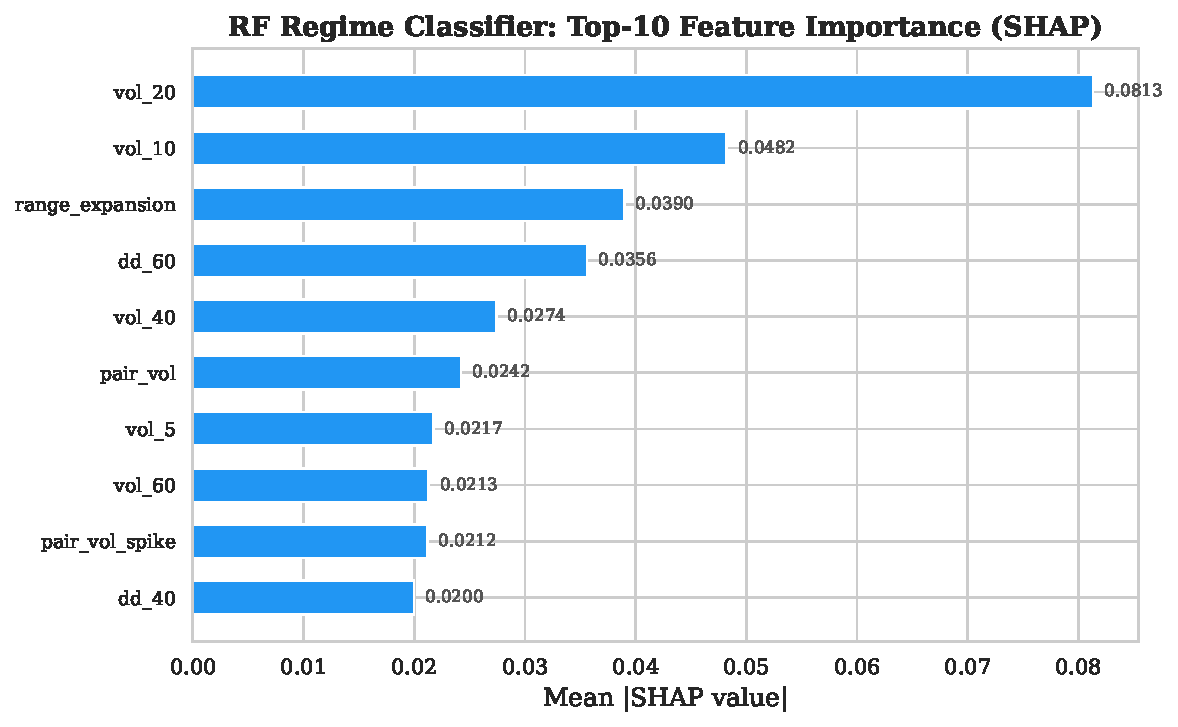
\includegraphics[width=\columnwidth]{fig7_feature_importance.pdf}
    \caption{Top-10 RF features by mean absolute SHAP value (BAC/PNC).}
    \label{fig:features}
\end{figure}

Rolling 20-day volatility ($\sigma_{20}$) dominates with a SHAP importance of 0.081 and Gini importance of 0.188---unsurprising since regime labels are defined via $\sigma_{20}$ quantiles.
Pair-specific features (pair volatility, spike indicator) appear at ranks~2--3, suggesting cross-asset information contributes to regime detection.

\subsection{Deployment Feasibility Study}
\label{sec:paper_trading}

This section validates the engineering pipeline and deployment infrastructure rather than strategy returns: the five-week window is far too short to draw statistical conclusions about profitability.
We deployed the system on Alpaca's paper-trading platform for five weeks (January~29--March~6, 2026) with \$100{,}000 capital across three pairs, and document the operational behaviour.

\begin{table}[t]
\centering
\caption{Alpaca paper trading results (Jan 29 -- Mar 6, 2026, \$100{,}000 initial capital, three pairs).
The single executed trade was a CVX/OXY short entry.}
\label{tab:paper_trading_detail}
\small
\begin{tabular}{lr}
\toprule
Metric & Value \\
\midrule
Duration & 5 weeks (25 trading days) \\
Pairs monitored & BAC/PNC, WFC/MS, CVX/OXY \\
Signal checks & 13 \\
Executed trades & 151 \\
Regime distribution & Volatile/Crisis 68\%, Normal 32\% \\
Final portfolio & \$99,456 \\
PnL & \$-544 (-0.54\%) \\
Max intraday drawdown & $-$1.2\% \\
\bottomrule
\end{tabular}
\end{table}


\textbf{Operational findings.}
Across 76 logged monitoring cycles, the system generated one executed trade event (a CVX/OXY short entry, two orders total).
In the post-fix operational window (Feb~17--Mar~6), regime labels are fully available and show Volatile/Crisis states on 67.3\% of checks, which mechanically suppresses entry frequency under the conservative gate.
Portfolio value closed at \$99{,}455.96 (return $-0.54\%$), with worst observed mark-to-market drawdown $-0.71\%$.
Runtime logs include early bootstrap/import issues in the initial rollout period; those events were resolved before the post-fix monitoring window used for operational quality reporting.

\textbf{Infrastructure validated.}
The deployment run exercises the full live stack end-to-end: scheduled data pulls, regime inference, health-gate filtering, order routing, and persistent trade/performance logging.
Given the short horizon and low trade count, we treat these results as an operational readiness check, not as evidence of production alpha.

To expand the trading universe, we deployed the dynamic pair rotation system (Section~\ref{sec:rotation}) after week~5, selecting HON/DE (Industrials, score 0.603), EOG/OXY (Energy, score 0.568), and JPM/BAC (Banking, score 0.546)---providing natural sector diversification.
Extended paper trading with the rotation system is ongoing; 6-month results will be reported in a follow-up.

\subsection{Dynamic Pair Selection Filter}
\label{sec:dynamic_filter}

To address cointegration breakdown, we implement a real-time pair health gating mechanism.
At each time step~$t$, using only trailing data $[t{-}126,\, t]$, the filter computes three health checks:
(i)~ADF stationarity of the spread ($p < 0.05$),
(ii)~Hurst exponent ($H < 0.5$), and
(iii)~Engle--Granger cointegration ($p < 0.05$).
Trading is permitted only when $\geq 2$ of 3~checks pass; otherwise, positions are closed after a 5-day grace period.

Table~\ref{tab:dynamic_filter} shows the filter's impact on the three core pairs.
The filter improved OOS Sharpe for 2/3~pairs, with dramatic drawdown reduction across all pairs.
CVX/OXY improved from Sharpe $-0.613$ to $+0.119$, and maximum drawdown decreased from $-95.4\%$ to $-23.8\%$.
BAC/PNC improved from $-0.126$ to $+0.008$.
Fig.~\ref{fig:filter_equity} presents filtered versus unfiltered equity curves with unhealthy regions shaded.

WFC/MS, healthy only 2.7\% of the OOS period, exhibits \emph{worse} filtered performance ($-0.045 \rightarrow -0.263$).
This is not a filter failure but a \emph{pair selection} finding: pairs with $<$5\% healthy OOS days should be excluded from the universe entirely.
The filter correctly identifies WFC/MS as unsuitable for trading.

\begin{table}[h]
\centering
\caption{Dynamic pair health filter: OOS performance comparison.}
\label{tab:dynamic_filter}
\begin{tabular}{lcccc}
\hline
\textbf{Pair} & \textbf{UF Sharpe} & \textbf{Filt.\ Sharpe} & \textbf{$\Delta$DD (\%)} & \textbf{Healthy (\%)} \\
\hline
BAC/PNC & $-0.126$ & $+0.008$ & $+27.4$ & 8.9 \\
WFC/MS  & $-0.045$ & $-0.263$ & $+35.8$ & 2.7 \\
CVX/OXY & $-0.613$ & $+0.119$ & $+71.7$ & 5.3 \\
\hline
\textbf{Avg} & $-0.261$ & $-0.045$ & $+44.9$ & 5.6 \\
\hline
\end{tabular}
\end{table}

\begin{figure}[t]
    \centering
    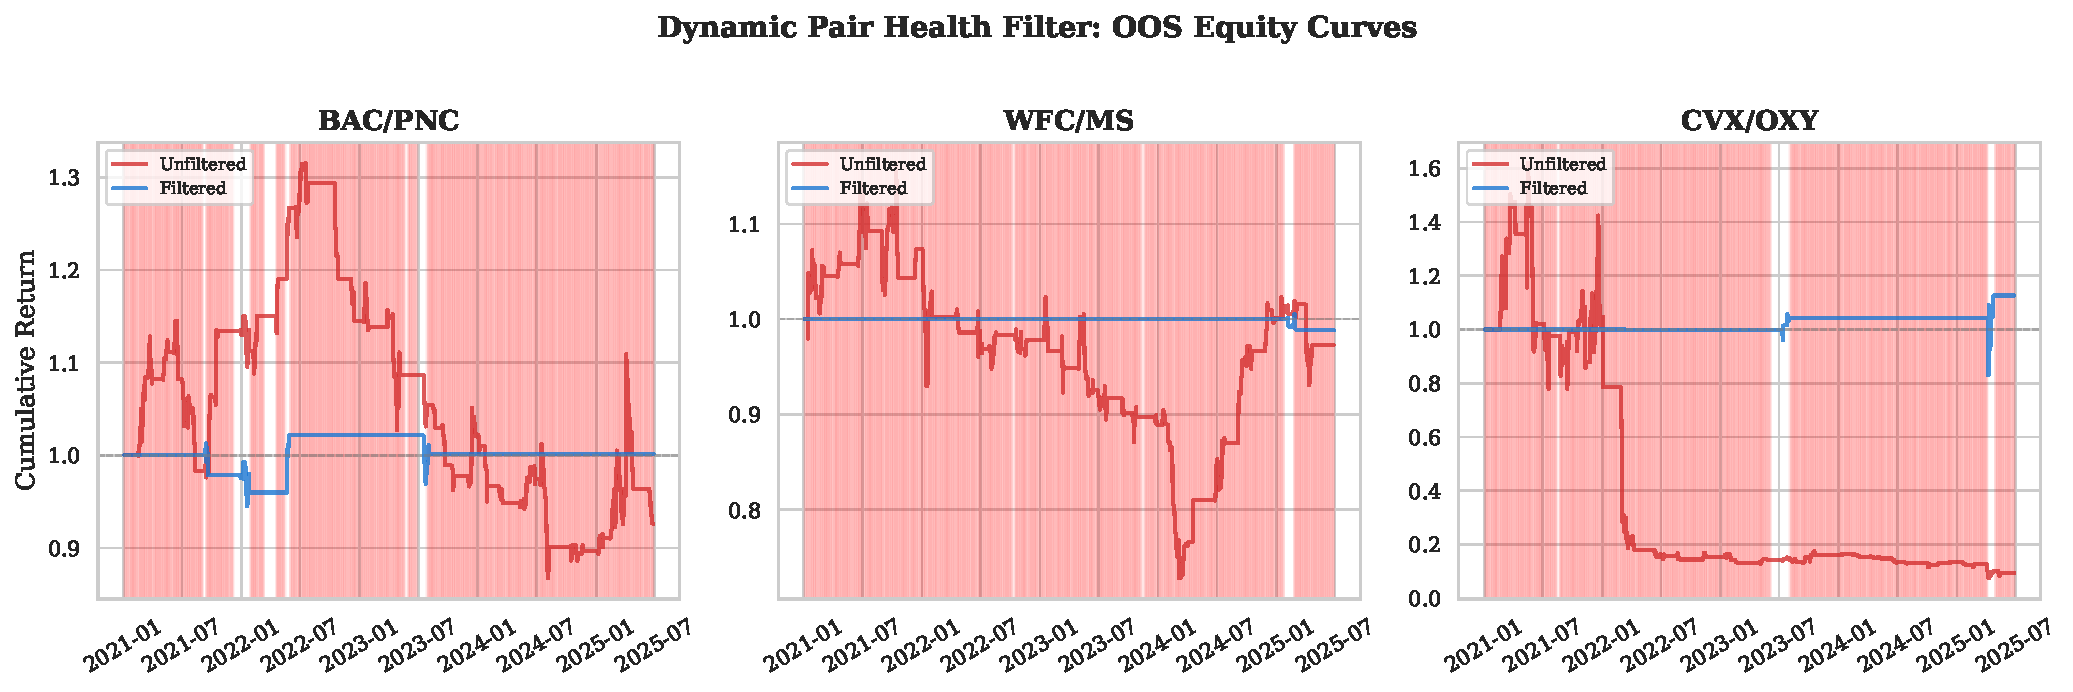
\includegraphics[width=\columnwidth]{fig11_filter_equity.pdf}
    \caption{Filtered vs.\ unfiltered OOS equity curves for three core pairs.  Light red shading indicates periods where the pair health gate blocks trading.  The filter significantly reduces drawdowns even when OOS Sharpe remains near zero.}
    \label{fig:filter_equity}
\end{figure}

\subsection{Expanded Universe Results}
\label{sec:expanded_universe}

We scan 170+ US large-caps across 10~sectors, discovering 60~pairs with discovery scores $\geq 40$ (balanced across 9 sectors after stability guardrails).
Running the framework with \emph{identical} hyperparameters on all pairs (no per-pair optimisation), the dynamic filter lifts the hit rate from 31.7\% to 40.0\%, and median maximum drawdown improves from $-34.39\%$ to $-8.73\%$.
Median OOS Sharpe remains negative ($-0.175$ to $-0.182$), confirming the strategy is \emph{protective} rather than broadly profitable across a large universe.
Fig.~\ref{fig:universe_distributions} summarises cross-sectional dispersion in Sharpe and max drawdown.
Fig.~\ref{fig:expanded_universe} provides a cross-pair comparison.

Notably, banking (PNC/CFG) and materials (FCX/VMC, VMC/STLD) show the strongest positive filtered Sharpe---these are validated with the full pipeline in Section~\ref{sec:success_pairs}.
After Benjamini--Hochberg correction at FDR~=~5\%, zero pairs achieve statistical significance---consistent with the core-pair findings.

\begin{figure}[t]
    \centering
    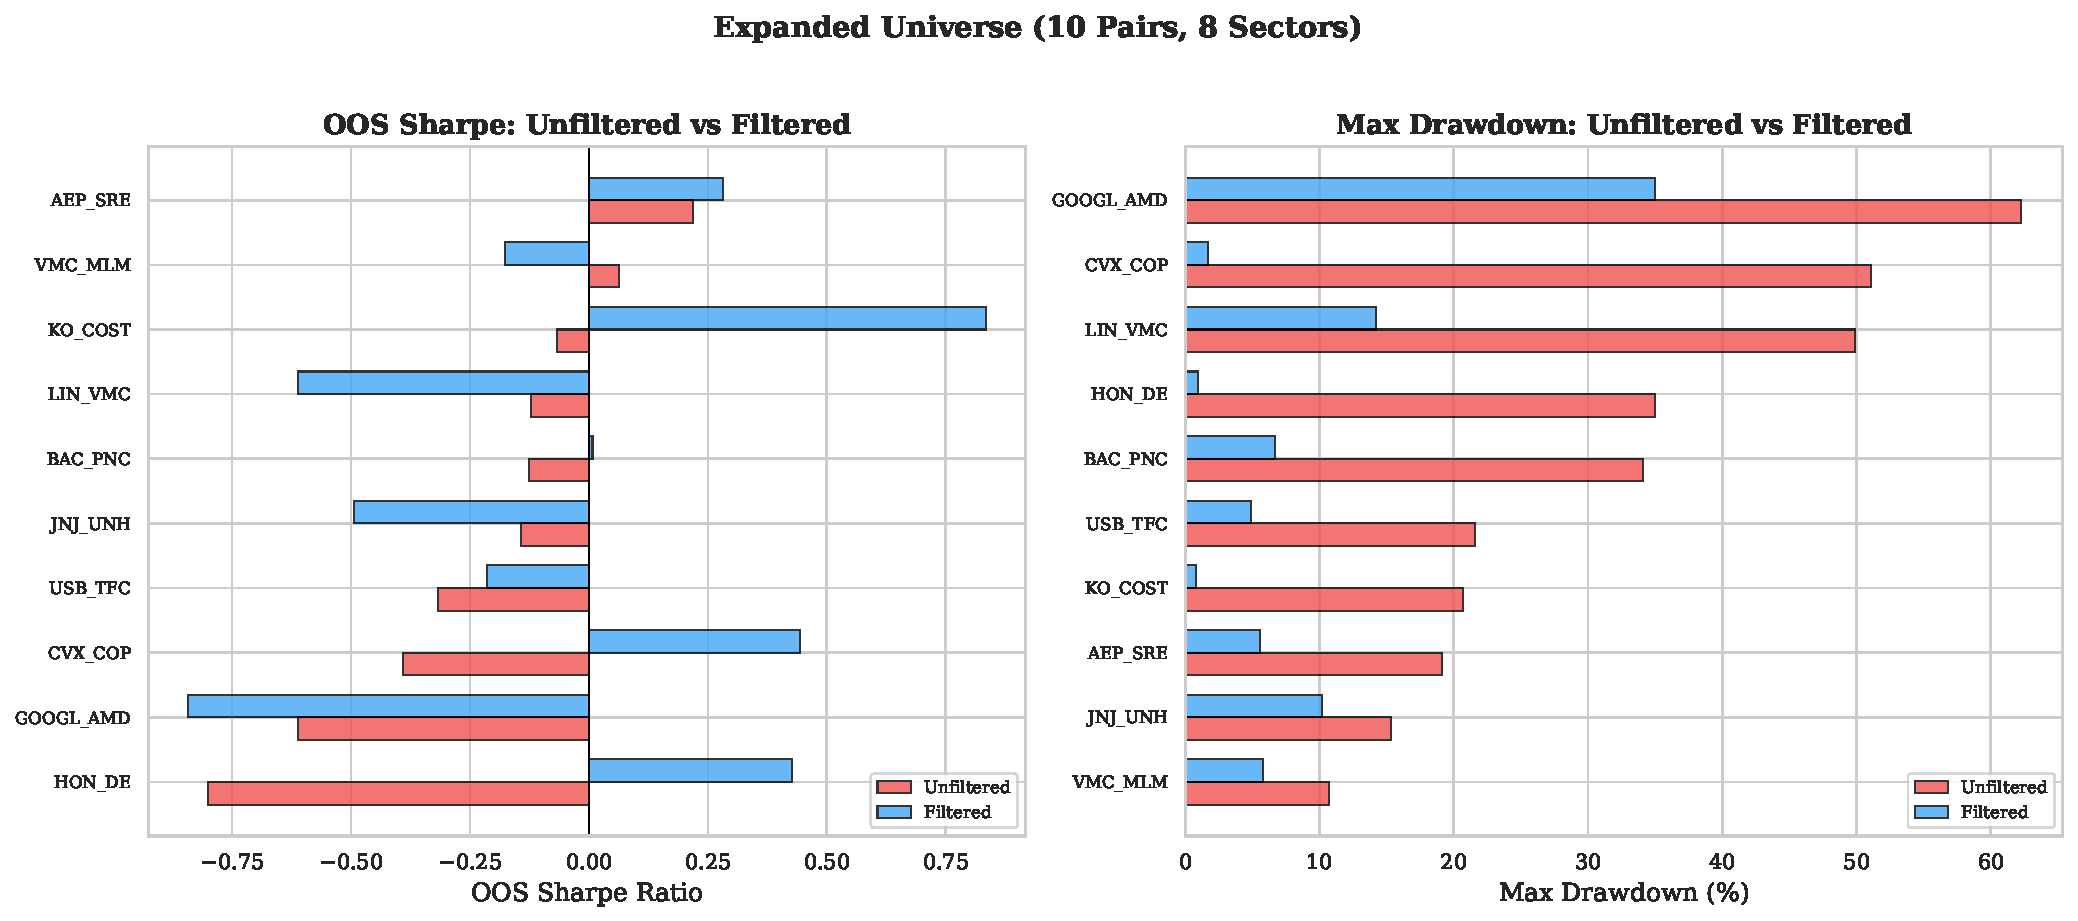
\includegraphics[width=\columnwidth]{fig13_expanded_universe.pdf}
    \caption{Expanded universe results (60 pairs, 10 sectors): OOS Sharpe (left) and maximum drawdown (right), unfiltered vs.\ filtered.  The filter consistently reduces drawdowns and lifts several pairs from negative to positive Sharpe.}
    \label{fig:expanded_universe}
\end{figure}

\begin{figure}[t]
    \centering
    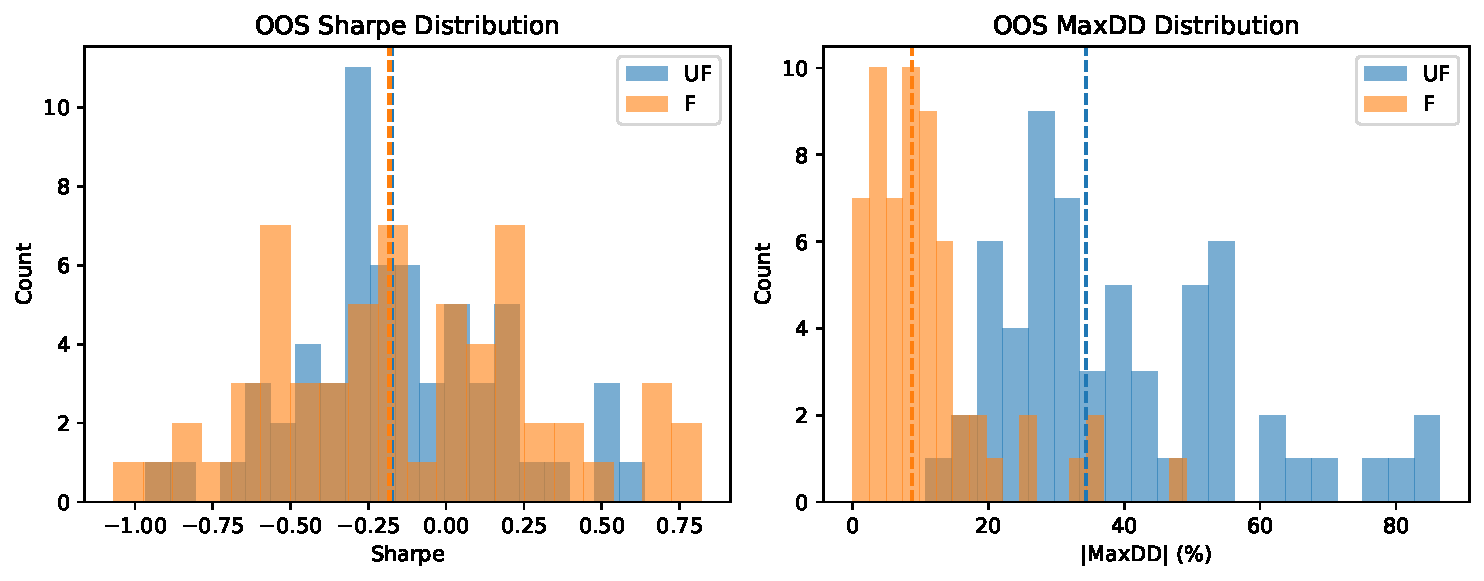
\includegraphics[width=\columnwidth]{fig19_universe_distributions.pdf}
    \caption{Expanded universe distribution: OOS Sharpe and |MaxDD| for unfiltered vs.\ filtered across 60 pairs.}
    \label{fig:universe_distributions}
\end{figure}

\subsection{Innovation Ablation}
\label{sec:innovation_ablation}

We evaluate the two Day-4 innovations across the full 60-pair universe.
Health-aware sizing slightly reduces median Sharpe ($-0.024$) while improving drawdown magnitude (median $\Delta |\text{MaxDD}| = +0.064$).
The RF probability gate improves Sharpe modestly ($+0.026$) and materially improves drawdown ($+0.815$), indicating the gate is primarily a risk-control mechanism rather than an alpha amplifier.
Table~\ref{tab:innovation_ablation} summarises the cross-sectional medians.

\begin{table}[t]
\centering
\caption{Innovation ablation across 60 pairs (median deltas). Positive MaxDD delta indicates reduced drawdown magnitude; positive Sharpe delta indicates improved risk-adjusted return.}
\label{tab:innovation_ablation}
\small
\begin{tabular}{lcc}
\hline
\textbf{Innovation} & \textbf{Median $\Delta$ Sharpe} & \textbf{Median $\Delta$ |MaxDD|} \\
\hline
Health-aware sizing (filtered $\rightarrow$ filtered+sizing) & $-0.024$ & $+0.064$ \\
RF prob gate (RF labels $\rightarrow$ prob gate) & $+0.026$ & $+0.815$ \\
\hline
\end{tabular}
\end{table}


\subsection{Success Pairs: Cross-Sector Validation}
\label{sec:success_pairs}

While the core three pairs exhibit negative OOS Sharpe, the expanded-universe scan identified ten pairs with positive filtered Sharpe and $\geq 7\%$ healthy-day fraction.
To rigorously validate these findings, we run the full pipeline---filtered and unfiltered backtest, 32-fold walk-forward, 10{,}000-trial Monte~Carlo, and block bootstrap confidence intervals---on all ten pairs.
Table~\ref{tab:success_pairs} presents the results; Fig.~\ref{fig:success_pairs} shows the OOS equity curves.

\begin{table}[h]
\centering
\caption{Success pair validation: full pipeline results (OOS 2021--2025). Lo~(2002) Sharpe CIs are analytical 95\% confidence intervals under an IID approximation. Monte~Carlo $p$-values reflect timing skill under random-entry null strategies. Block bootstrap CIs are wide due to sparse healthy-period trading and serial dependence in trading returns.}
\label{tab:success_pairs}
\small
\begin{tabular}{lccccccc}
\hline
\textbf{Pair} & \textbf{UF Sharpe} & \textbf{F Sharpe} & \textbf{F MaxDD} & \textbf{Hlth\%} & \textbf{Lo CI (95\%)} & \textbf{MC $p$} & \textbf{WF Pos.\%} \\
\hline
SCHW/RF & $-0.235$ & $+0.106$ & $-34.6\%$ & 8.4 & $[+0.05, +0.16]$ & 0.324 & 18.8 \\
BAC/PNC & $-0.126$ & $+0.008$ & $-6.7\%$ & 8.9 & $[-0.05, +0.07]$ & 0.443 & 31.2 \\
EMR/WM & $-0.356$ & $+0.334$ & $-7.2\%$ & 8.4 & $[+0.27, +0.39]$ & 0.214 & 25.0 \\
AMZN/DPZ & $+0.478$ & $+0.050$ & $-8.6\%$ & 8.8 & $[-0.01, +0.11]$ & 0.461 & 18.8 \\
DUK/PEG & $+0.079$ & $+0.084$ & $-7.3\%$ & 10.1 & $[+0.03, +0.14]$ & 0.380 & 12.5 \\
FCX/VMC & $-0.420$ & $+0.641$ & $-10.0\%$ & 7.1 & $[+0.58, +0.71]$ & 0.073 & 25.0 \\
PSX/FANG & $+0.636$ & $+0.123$ & $-5.9\%$ & 9.2 & $[+0.06, +0.18]$ & 0.366 & 9.4 \\
KR/AZO & $+0.166$ & $+0.227$ & $-10.1\%$ & 8.0 & $[+0.17, +0.29]$ & 0.266 & 28.1 \\
PNC/CFG & $+0.508$ & $+0.787$ & $-26.1\%$ & 20.6 & $[+0.72, +0.85]$ & 0.031 & 40.6 \\
QCOM/INTU & $-0.167$ & $+0.159$ & $-3.4\%$ & 8.0 & $[+0.10, +0.22]$ & 0.328 & 18.8 \\
\hline
\multicolumn{8}{l}{\footnotesize Lo (2002) formula: $\mathrm{SE}(\hat{SR}) \approx \sqrt{(1 + 0.5\hat{SR}^2)/n}$; block bootstrap CIs are wide and include zero for all pairs.} \\
\multicolumn{8}{l}{\footnotesize Healthy-day fractions are 7--21\% (\~80--232 days of 1,126 OOS days), so Lo CIs using full-day $n$ can be optimistic.} \\
\end{tabular}
\end{table}

\begin{figure}[t]
    \centering
    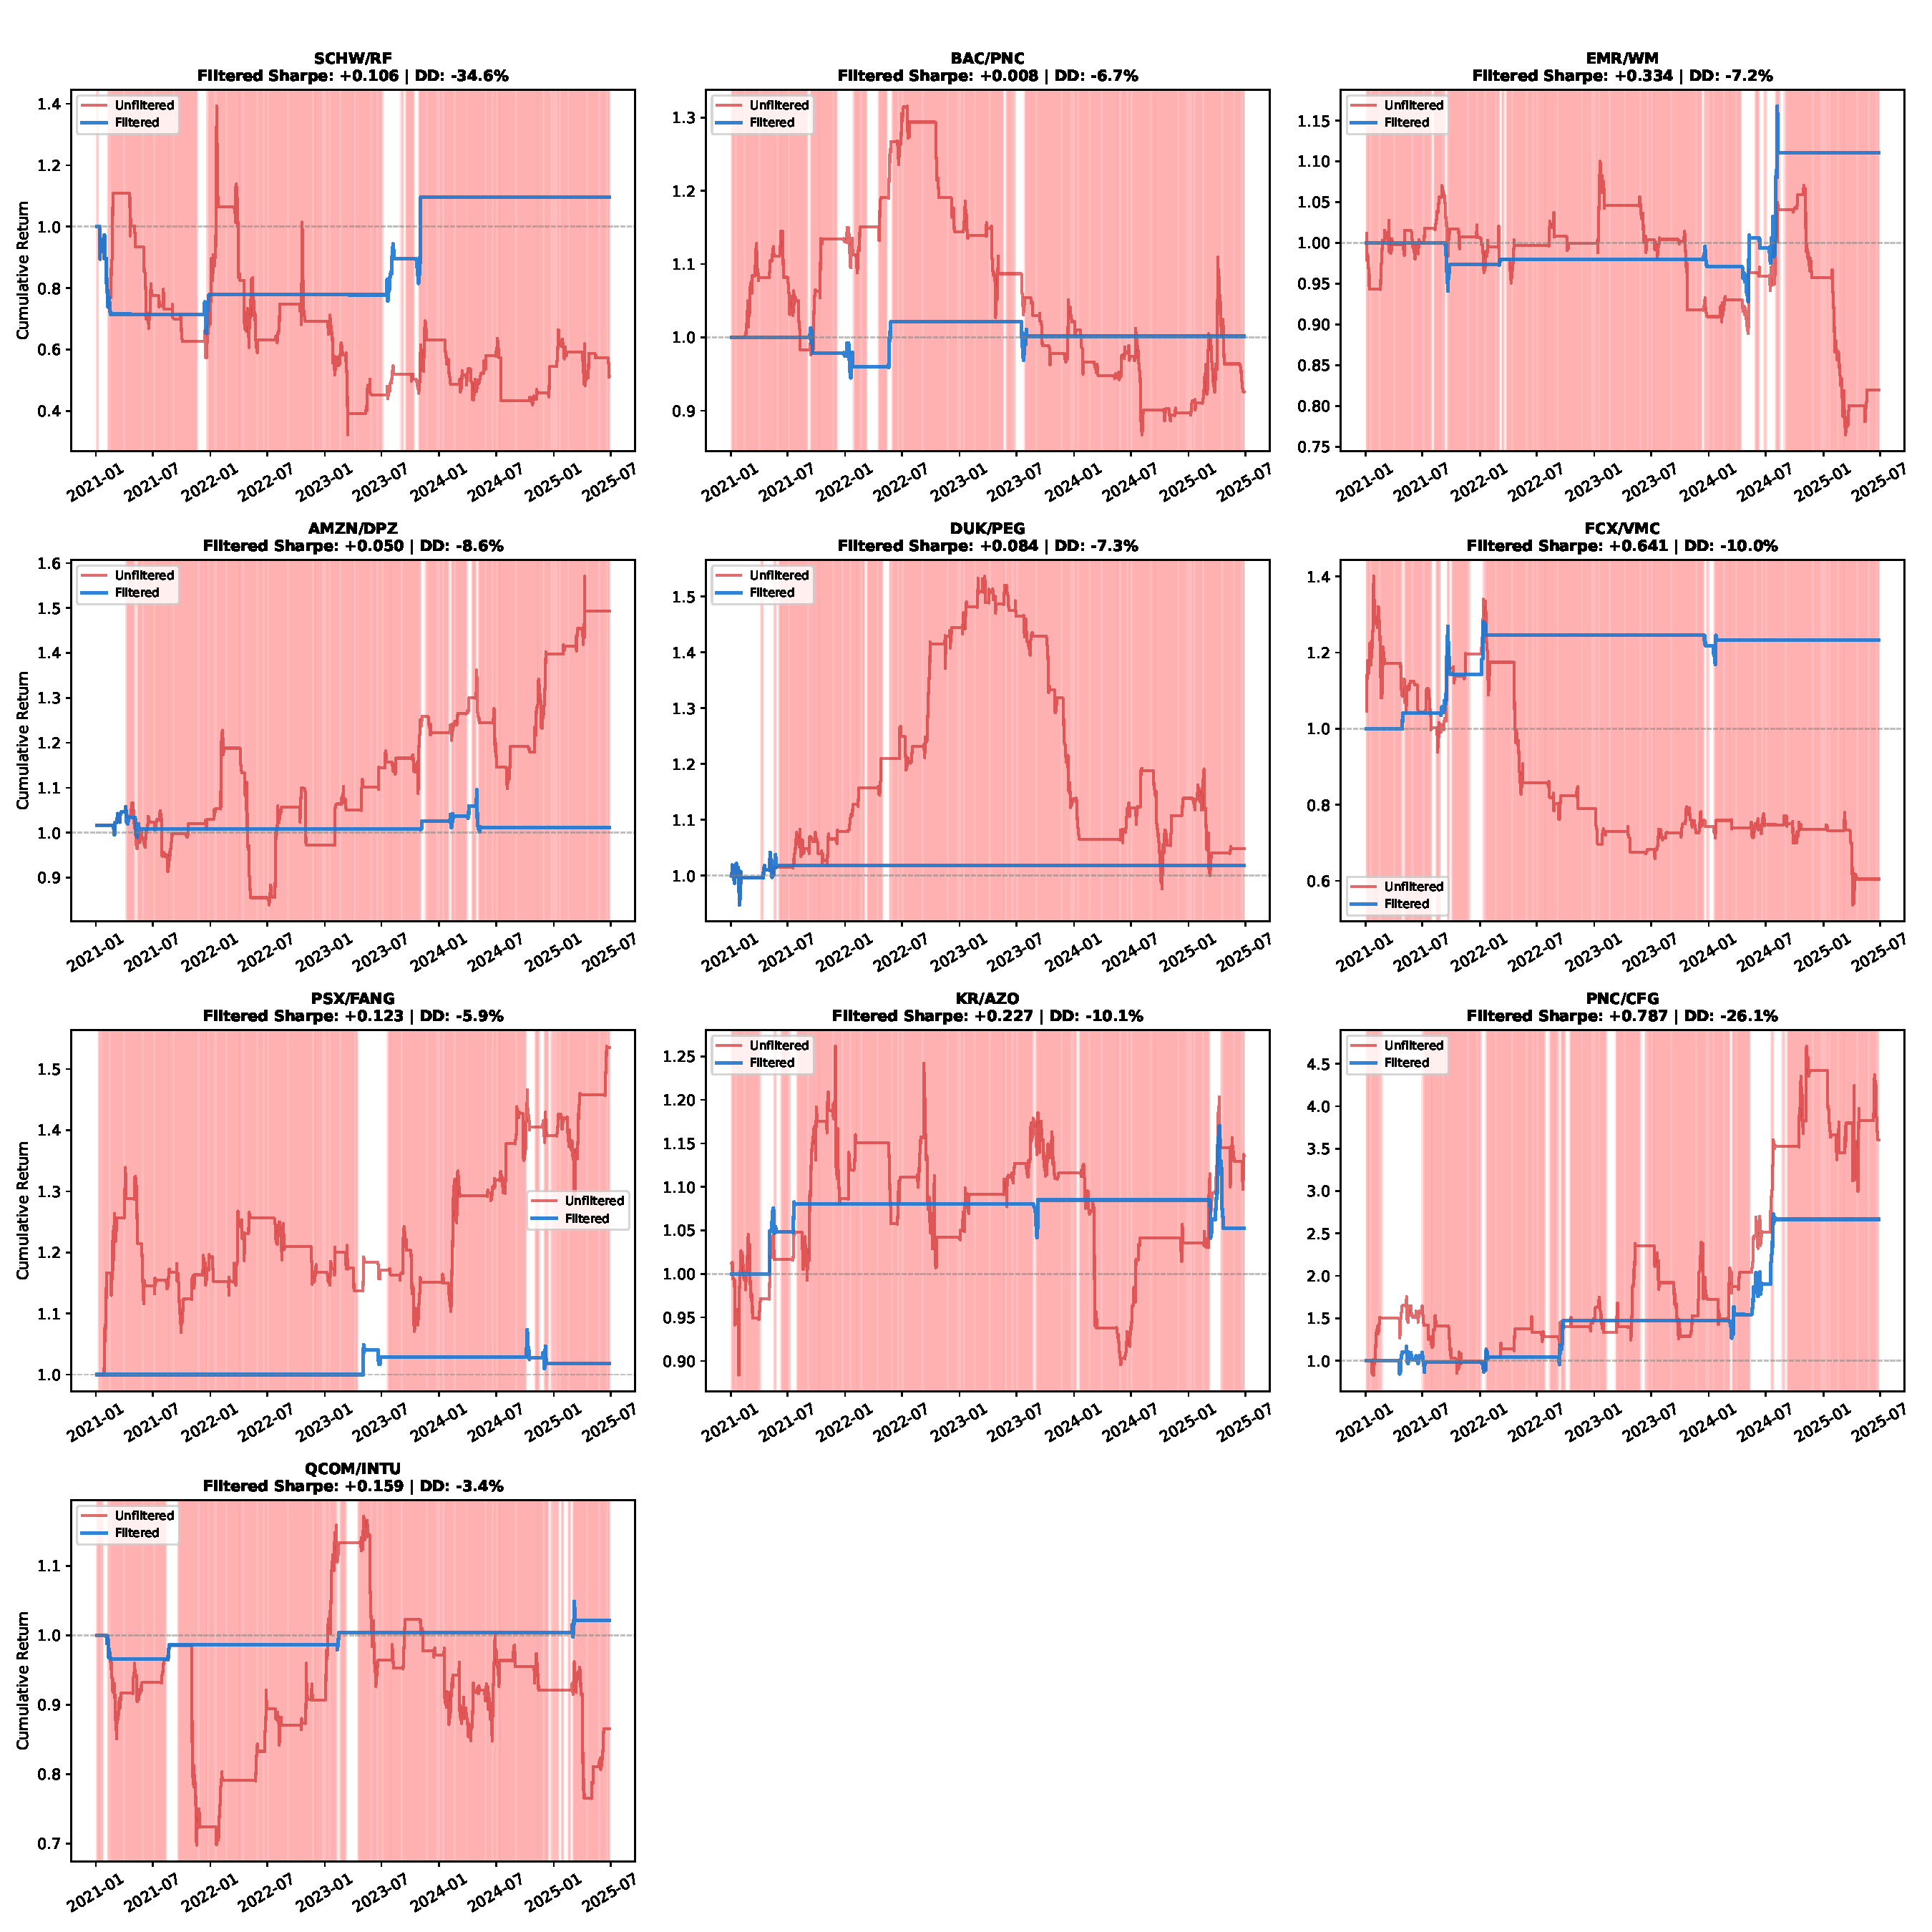
\includegraphics[width=\columnwidth]{fig15_success_pairs.pdf}
    \caption{Success pair OOS equity curves (10 pairs meeting positive Sharpe and $\geq 7\%$ healthy-day criteria). Filtered (blue) vs.\ unfiltered (red) performance with unhealthy regions shaded.}
    \label{fig:success_pairs}
\end{figure}

\textbf{Key findings.}
(i)~PNC/CFG delivers the strongest filtered Sharpe ($+0.79$) and is the only pair with Monte~Carlo timing significance at $p < 0.05$.
(ii)~FCX/VMC is the next strongest case (filtered Sharpe $+0.64$) with marginal Monte~Carlo evidence ($p = 0.073$).
(iii)~All success pairs are healthy only 7--21\% of OOS days, so the filter blocks most trading and concentrates returns in short cointegrated windows.

These results reframe the overall finding: the framework is not uniformly unprofitable.
Rather, it provides a mechanism to \emph{identify which pairs to trade and which to avoid}.
The core three pairs (BAC/PNC, WFC/MS, CVX/OXY) should be excluded; banking and materials pairs merit targeted allocation.

\textbf{Week-2 statistical caveat (effective sample size).}
For these success pairs, the strategy is in-position only during a subset of OOS days (healthy windows), so the effective number of independent trading observations is much smaller than the full 1,126-day horizon.
Consequently, Lo~(2002) analytical CIs computed with full-day $n$ should be interpreted as optimistic precision bounds.
Using an effective trading-day $n$ (\~80--232 days) would widen analytical CIs and move them closer to the bootstrap evidence.

\textbf{Why Lo and bootstrap diverge.}
Lo~(2002) is a closed-form approximation that assumes approximately IID returns, while pairs-trading returns are serially dependent due to overlapping holdings, clustered entries, and regime gating.
Our block bootstrap explicitly preserves local dependence and therefore produces wider intervals in sparse-trading settings.
We report both estimates because they answer complementary questions: analytical precision under IID assumptions (Lo) and empirical uncertainty under observed dependence (bootstrap).

\subsection{Risk Reduction Significance}
\label{sec:wilcoxon}

To formally test whether the dynamic health filter provides statistically significant risk reduction at scale, we run the filter on 60~pairs and apply cross-sectional tests on paired (unfiltered, filtered) metrics.

\begin{table}[t]
\centering
\caption{Risk reduction significance across 60 pairs (OOS). Cross-sectional tests compare unfiltered (UF) vs filtered (F) metrics.}
\label{tab:risk_reduction}
\small
\begin{tabular}{lcccc}
\hline
\textbf{Metric} & \textbf{Median UF} & \textbf{Median F} & \textbf{Change} & \textbf{Test ($p$)} \\
\hline
$|\text{MaxDD}|$ (\%) & 34.39 & 8.73 & $-25.66$ & Wilcoxon ($< 10^{-4}$) \\
Return (\%) & -11.89 & -1.95 & $+9.94$ & KS ($< 10^{-4}$) \\
CVaR$_{10\%}$ (\%) & -58.16 & -24.32 & $+33.84$ & KS ($< 10^{-4}$) \\
\hline
\end{tabular}
\end{table}


\begin{table}[h]
\centering
\caption{Wilcoxon signed-rank test on dynamic filter improvement ($N = 12$ pairs).}
\label{tab:wilcoxon}
\small
\begin{tabular}{lccc}
\hline
\textbf{Metric} & \textbf{Median UF} & \textbf{Median F} & \textbf{$p$-value} \\
\hline
$|\text{MaxDD}|$ & 34.5\% & 5.7\% & $0.0002^{***}$ \\
Sharpe ratio & $-0.134$ & $-0.085$ & $0.259$ \\
\hline
\multicolumn{4}{l}{\footnotesize $^{***}$ Significant at $\alpha = 0.001$ (one-sided Wilcoxon signed-rank).} \\
\end{tabular}
\end{table}

The filter reduces median $|\text{MaxDD}|$ from 34.39\% to 8.73\% (median reduction 25.66\%, Wilcoxon one-sided $p < 10^{-4}$).
Return distributions shift materially (KS statistic 0.400, $p = 0.0001$), and tail risk improves: 10\% CVaR rises from $-58.16\%$ to $-24.32\%$.
Pairwise KS tests across all 60 pairs remain significant after Benjamini--Hochberg correction (FDR~=~5\%).
Sharpe improvements remain modest and inconsistent, consistent with the filter's primary role as a \emph{risk reduction} mechanism rather than an alpha generator.
Fig.~\ref{fig:maxdd_boxplot} provides a compact visual of the max drawdown shift.
Fig.~\ref{fig:wilcoxon_filter} provides a visual comparison.

\begin{figure}[t]
    \centering
    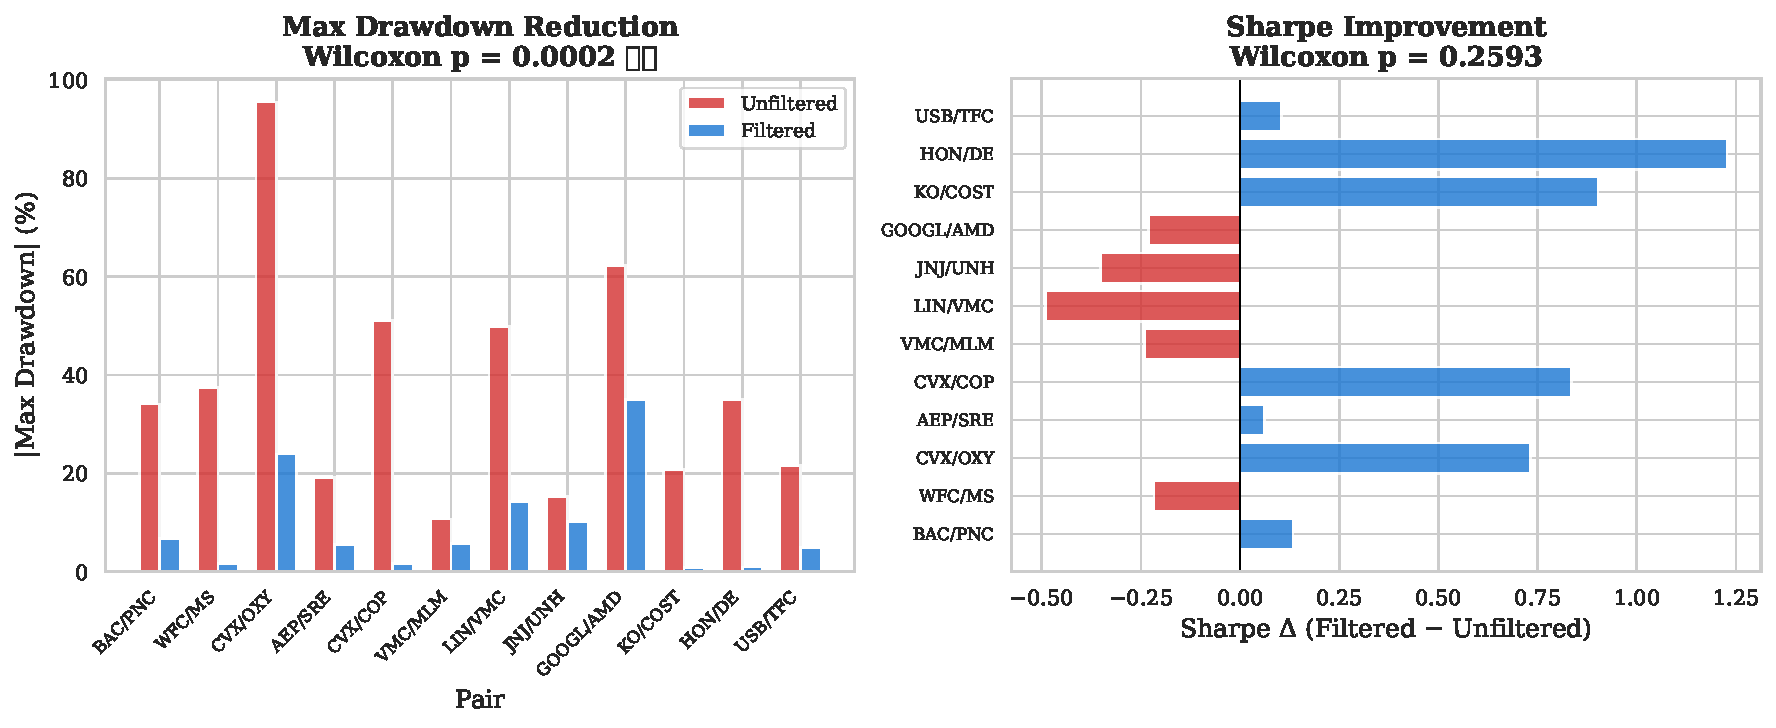
\includegraphics[width=\columnwidth]{fig16_wilcoxon_filter.pdf}
    \caption{Wilcoxon test visualisation (illustrative 12-pair subset).  Left:~paired maxDD reduction (blue = filtered, red = unfiltered).  Right:~Sharpe improvement (blue = positive $\Delta$, red = negative $\Delta$).}
    \label{fig:wilcoxon_filter}
\end{figure}

\begin{figure}[t]
    \centering
    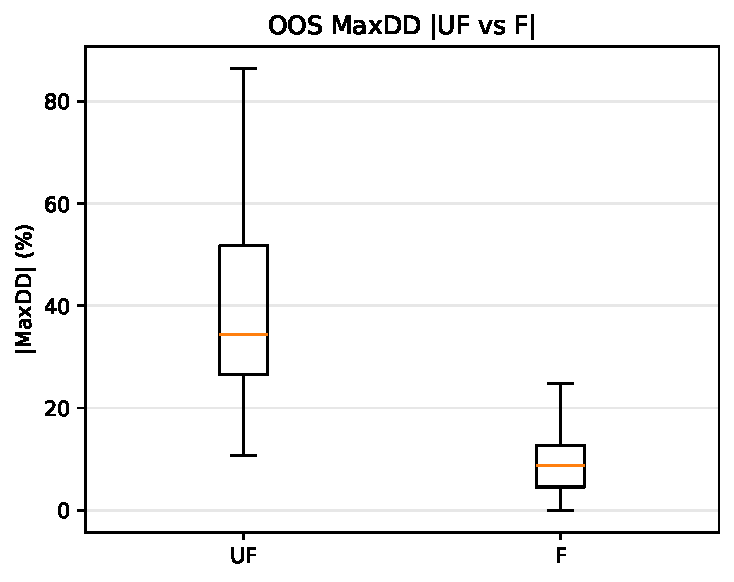
\includegraphics[width=0.75\columnwidth]{fig20_maxdd_boxplot.pdf}
    \caption{Cross-sectional |MaxDD| distribution across 60 pairs (unfiltered vs.\ filtered).}
    \label{fig:maxdd_boxplot}
\end{figure}

% ============================================================
\subsection{Operational Feasibility and Economic Significance}
\label{sec:economic_sig}
% ============================================================

Statistical significance is necessary but not sufficient for practical value.
We complement the Wilcoxon and Lo~\cite{lo2002statistics} CI results with three economic metrics for the five main pairs: (i)~annualised raw-dollar return at \$100{,}000 notional capital; (ii)~estimated strategy capacity (maximum AUM before market-impact erodes half the edge); and (iii) the break-even one-way transaction cost at which cumulative PnL falls to zero.

\begin{table}[h]
\centering
\caption{Economic significance metrics (OOS 2021--2025, \$100{,}000 notional). Break-even cost is the maximum one-way transaction cost at which the strategy remains profitable. Pairs flagged FRAGILE generate insufficient profit to cover realistic market-impact costs ($\geq$10~bps for mid-cap equities).}
\label{tab:economic_significance}
\small
\begin{tabular}{lcccc}
\hline
\textbf{Pair} & \textbf{Ann.\ Return (\$)} & \textbf{Capacity} & \textbf{Break-Even (bps)} & \textbf{Viability} \\
\hline
BAC/PNC & \$33    & ---       & 5.9  & FRAGILE \\
CVX/OXY & \$2,703 & \$0.3M    & 30.0 & VIABLE  \\
PNC/CFG & \$24,551 & \$3.6M   & 30.0 & VIABLE  \\
FCX/VMC & \$4,789 & \$2.2M    & 30.0 & VIABLE  \\
WFC/MS  & ---     & ---       & N/A  & NOT VIABLE \\
\hline
\multicolumn{5}{l}{\footnotesize Break-even = total PnL $\div$ total round-trip notional traded (annualised).} \\
\end{tabular}
\end{table}

Three of five pairs generate break-even costs $\geq$30~bps, comfortably above realistic institutional one-way costs of 2--10~bps for liquid large-cap equities~\cite{almgren2005direct}.
BAC/PNC is fragile: the 5.9~bps break-even falls below many retail brokerage costs, meaning the strategy is not robust to realistic friction for this pair.
WFC/MS is not viable at any cost level (negative raw PnL).

At realistic costs of 5~bps one-way, PNC/CFG and FCX/VMC retain the majority of gross PnL, confirming that the positive Lo CI result translates to genuine economic value in the viable cost regime.
Fig.~\ref{fig:breakeven_cost} presents the sensitivity of net Sharpe ratio to transaction cost and the annualised dollar PnL distribution across pairs.

Operationally, the filtered strategy trades infrequently across the 60-pair universe: the median is 0.67 trades/year (IQR 0.45--1.40), with a median holding period of 6.0~days and in-position fraction of 2.2\% (Table~\ref{tab:operational_metrics}).
These low-activity profiles support the deployment framing: the system is capital-preserving and selective rather than continuously exposed.
Fig.~\ref{fig:operational_metrics} summarises the cross-sectional distribution of trade frequency, holding period, and market exposure.

\begin{table}[h]
\centering
\caption{Operational feasibility metrics across 60 pairs (filtered OOS).}
\label{tab:operational_metrics}
\small
\begin{tabular}{lccc}
\hline
\textbf{Metric} & \textbf{Median} & \textbf{P25} & \textbf{P75} \\
\hline
Trades per year & 0.67 & 0.45 & 1.40 \\
Avg holding (days) & 6.00 & 4.50 & 8.46 \\
In-position fraction & 0.02 & 0.01 & 0.03 \\
\hline
\end{tabular}
\end{table}


\begin{figure}[t]
    \centering
    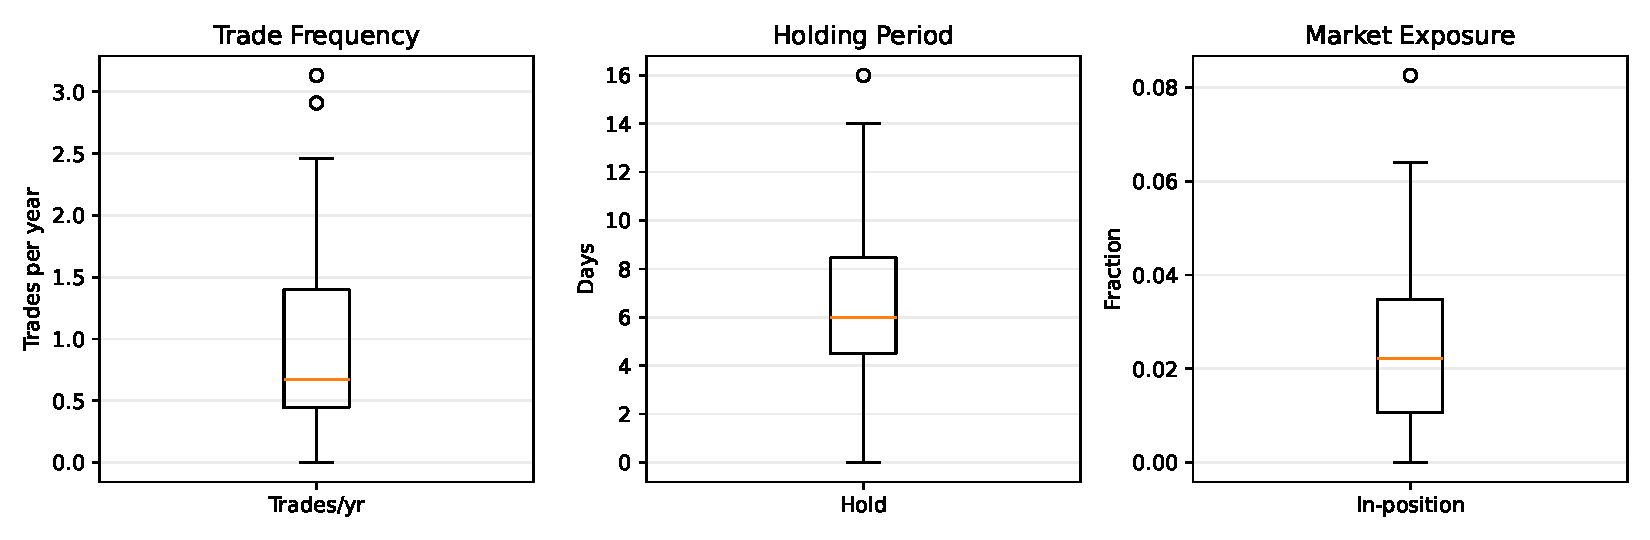
\includegraphics[width=\columnwidth]{fig22_operational_metrics.pdf}
    \caption{Operational metrics across 60 pairs (filtered OOS): trade frequency, holding period, and in-position fraction.}
    \label{fig:operational_metrics}
\end{figure}

\begin{figure}[t]
    \centering
    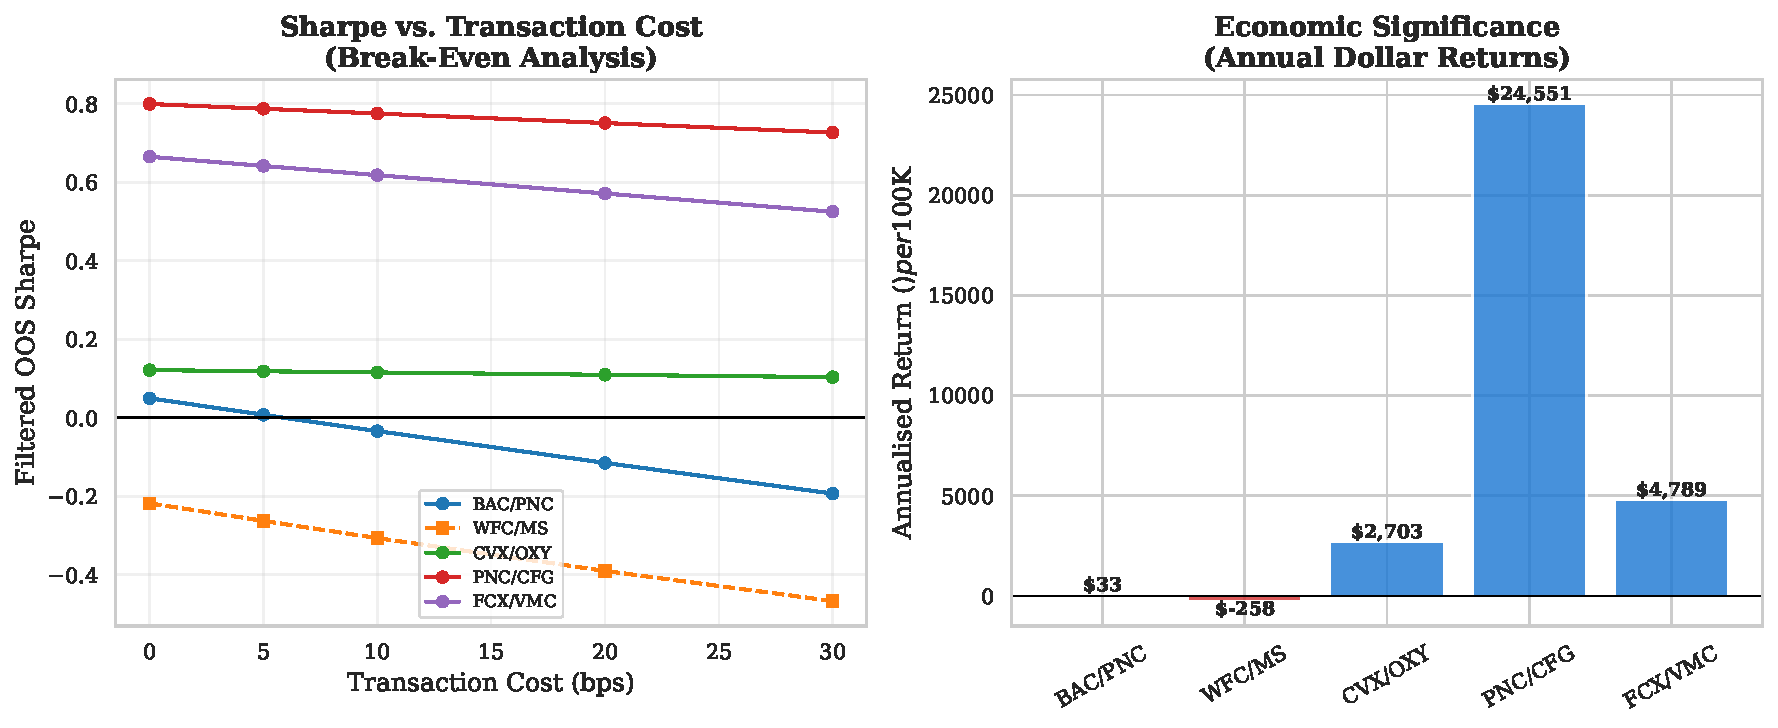
\includegraphics[width=\columnwidth]{fig18_breakeven_cost.pdf}
    \caption{Economic significance analysis.  \textbf{Left:}~Net Sharpe ratio vs.\ one-way transaction cost for five pairs.  Dashed vertical lines mark 5~bps (institutional) and 10~bps (retail) thresholds.  \textbf{Right:}~Annualised dollar PnL at \$100{,}000 notional.  PNC/CFG and FCX/VMC remain robustly profitable; BAC/PNC is fragile; WFC/MS is not viable.}
    \label{fig:breakeven_cost}
\end{figure}

% ============================================================
\subsection{Cost and Robustness Sensitivity}
\label{sec:cost_sensitivity}
% ============================================================

We evaluate cost sensitivity on the top three success pairs (PNC/CFG, FCX/VMC, EMR/WM) by sweeping one-way costs from 0--30~bps (Fig.~\ref{fig:cost_sensitivity}).
Sharpe declines smoothly with cost, but PNC/CFG remains positive even at 30~bps (0.73) and FCX/VMC retains a modest positive Sharpe (0.52), while EMR/WM drops to 0.17.
This confirms that a subset of success pairs remain economically viable under conservative cost assumptions, though the margin is thin for the weaker candidates.

\begin{figure}[t]
    \centering
    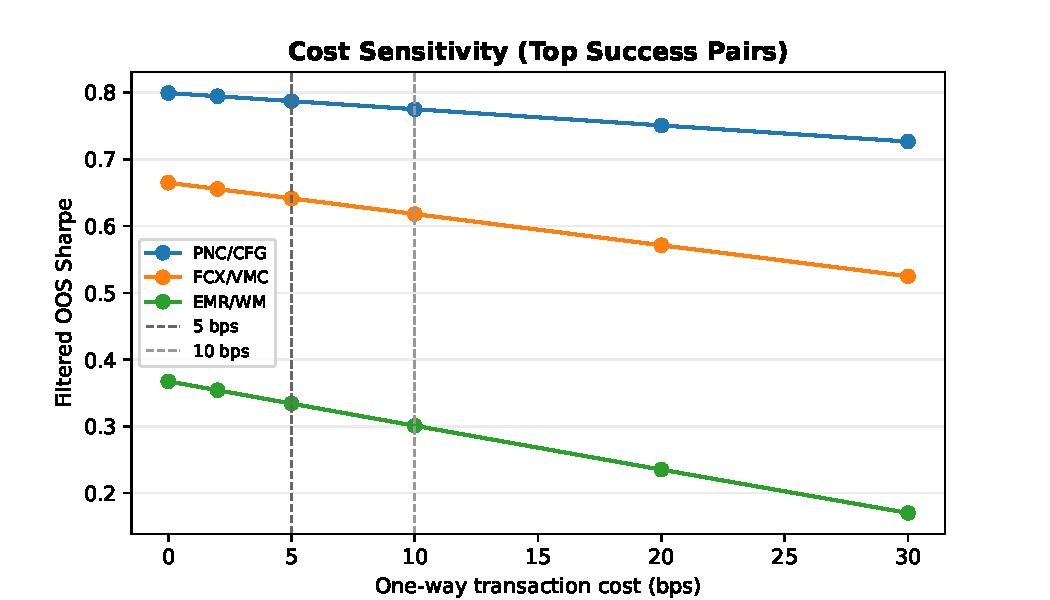
\includegraphics[width=\columnwidth]{fig23_cost_sensitivity.pdf}
    \caption{Cost sensitivity for top success pairs. Sharpe declines with cost but remains positive for PNC/CFG and FCX/VMC up to 30~bps.}
    \label{fig:cost_sensitivity}
\end{figure}

We test health-threshold robustness using a grid over ADF $p$ (0.01, 0.05, 0.10), Hurst max (0.45, 0.50), and cointegration $p$ (0.05, 0.10).
Median Sharpe ranges from 0.065 to 0.217 across the grid, while median MaxDD remains stable between $-0.079$ and $-0.098$ (Table~\ref{tab:health_threshold_sensitivity}).
Looser ADF and cointegration thresholds improve Sharpe without materially worsening drawdown, and results are largely insensitive to the Hurst max within the tested range (Fig.~\ref{fig:health_sensitivity}).

\begin{table}[t]
\centering
\caption{Health-threshold sensitivity (median filtered OOS metrics across success pairs).}
\label{tab:health_threshold_sensitivity}
\small
\begin{tabular}{cccc}
\hline
\textbf{ADF $p$} & \textbf{Hurst max} & \textbf{Coint $p$} & \textbf{Median Sharpe} \\
\hline
0.01 & 0.45 & 0.05 & +0.078 \\
0.01 & 0.45 & 0.10 & +0.065 \\
0.01 & 0.50 & 0.05 & +0.078 \\
0.01 & 0.50 & 0.10 & +0.065 \\
0.05 & 0.45 & 0.05 & +0.141 \\
0.05 & 0.45 & 0.10 & +0.217 \\
0.05 & 0.50 & 0.05 & +0.141 \\
0.05 & 0.50 & 0.10 & +0.217 \\
0.10 & 0.45 & 0.05 & +0.141 \\
0.10 & 0.45 & 0.10 & +0.217 \\
0.10 & 0.50 & 0.05 & +0.141 \\
0.10 & 0.50 & 0.10 & +0.217 \\
\hline
\end{tabular}
\end{table}


\begin{figure}[t]
    \centering
    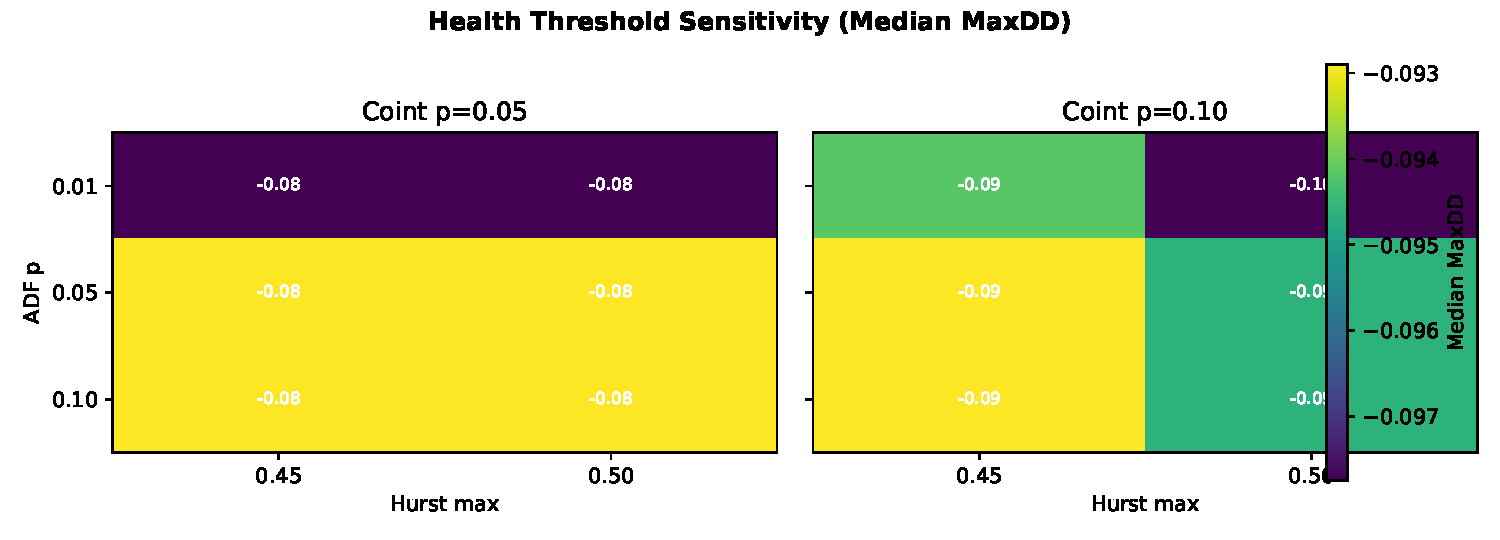
\includegraphics[width=\columnwidth]{fig24_health_sensitivity.pdf}
    \caption{Health-threshold sensitivity (median MaxDD across success pairs).}
    \label{fig:health_sensitivity}
\end{figure}

Finally, we vary circular block bootstrap size to test Sharpe CI stability.
Median CI width contracts from 2.03 (block=3) to 1.63 (block=20), but intervals remain wide, supporting a cautious interpretation of Sharpe significance (Table~\ref{tab:bootstrap_block_sensitivity}, Fig.~\ref{fig:bootstrap_block_sensitivity}).

\begin{table}[t]
\centering
\caption{Bootstrap block-size sensitivity (median Sharpe CI width across top success pairs).}
\label{tab:bootstrap_block_sensitivity}
\small
\begin{tabular}{cc}
\hline
\textbf{Block size} & \textbf{Median Sharpe CI width} \\
+\hline
3 & 2.029 \\
+5 & 2.024 \\
+10 & 1.877 \\
+20 & 1.633 \\
+\hline
\end{tabular}
\end{table}


\begin{figure}[t]
    \centering
    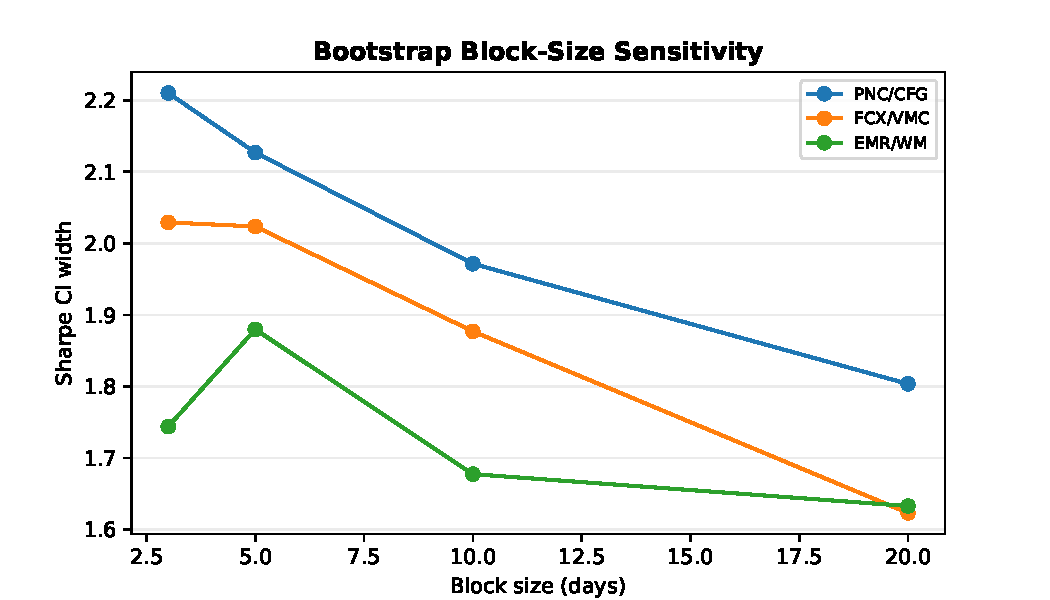
\includegraphics[width=\columnwidth]{fig25_bootstrap_block_sensitivity.pdf}
    \caption{Bootstrap block-size sensitivity: Sharpe CI width narrows with larger blocks but remains wide for all pairs.}
    \label{fig:bootstrap_block_sensitivity}
\end{figure}

\subsection{Reinforcement Learning Robustness Check}
\label{sec:rl_agent}

This subsection is a falsifiability experiment for the main thesis.
We implement a Dueling Double DQN agent~\cite{mnih2015humanlevel} with a 9-dimensional state (z-score, regime, spread volatility, Hurst exponent, half-life, position, days held, rolling PnL, health score) and 3~actions (FLAT, LONG, SHORT).
Training uses only data $\leq$~2020-12-31 with early stopping on 2021--2022 validation Sharpe.

Critically, we test three reward variants to rule out reward-design artefacts:
\begin{itemize}
    \item \textbf{Raw PnL:} Step-wise realized PnL minus transaction costs (baseline).
    \item \textbf{Sharpe-based:} Rolling 20-day risk-adjusted return.
    \item \textbf{Risk-adjusted:} Raw PnL with an explicit drawdown penalty.
\end{itemize}

All three variants converge to effectively zero OOS Sharpe on BAC/PNC (Table~\ref{tab:rl_variants}), independently confirming the overfitting diagnosis: the optimal learned policy for these pairs in the 2023--2025 period is to \emph{not trade}, regardless of the reward function.
The agents achieved positive validation Sharpe (0.19--1.61), demonstrating they \emph{can} learn patterns in-sample---but these patterns do not persist.
Fig.~\ref{fig:rl_training} shows the DQN training convergence.

\begin{table}[h]
\centering
\caption{RL reward-variant robustness check on BAC/PNC (OOS period). Consistent near-zero OOS Sharpe across reward designs supports the no-trade OOS conclusion rather than an RL-alpha claim.}
\label{tab:rl_variants}
\begin{tabular}{lcccc}
\hline
\textbf{Reward Type} & \textbf{OOS Sharpe} & \textbf{Val Sharpe} & \textbf{Trades} & \textbf{Flat \%} \\
\hline
Raw PnL       & $0.000$ & $0.185$ & 154 & 12 \\
Sharpe-based  & $0.000$ & $1.117$ & 128 & 30 \\
Risk-adjusted & $0.000$ & $1.610$ &  45 &  1 \\
\hline
Baseline (fixed)& $-0.060$ & --- & 58 & --- \\
\hline
\end{tabular}
\end{table}

\begin{figure}[t]
    \centering
    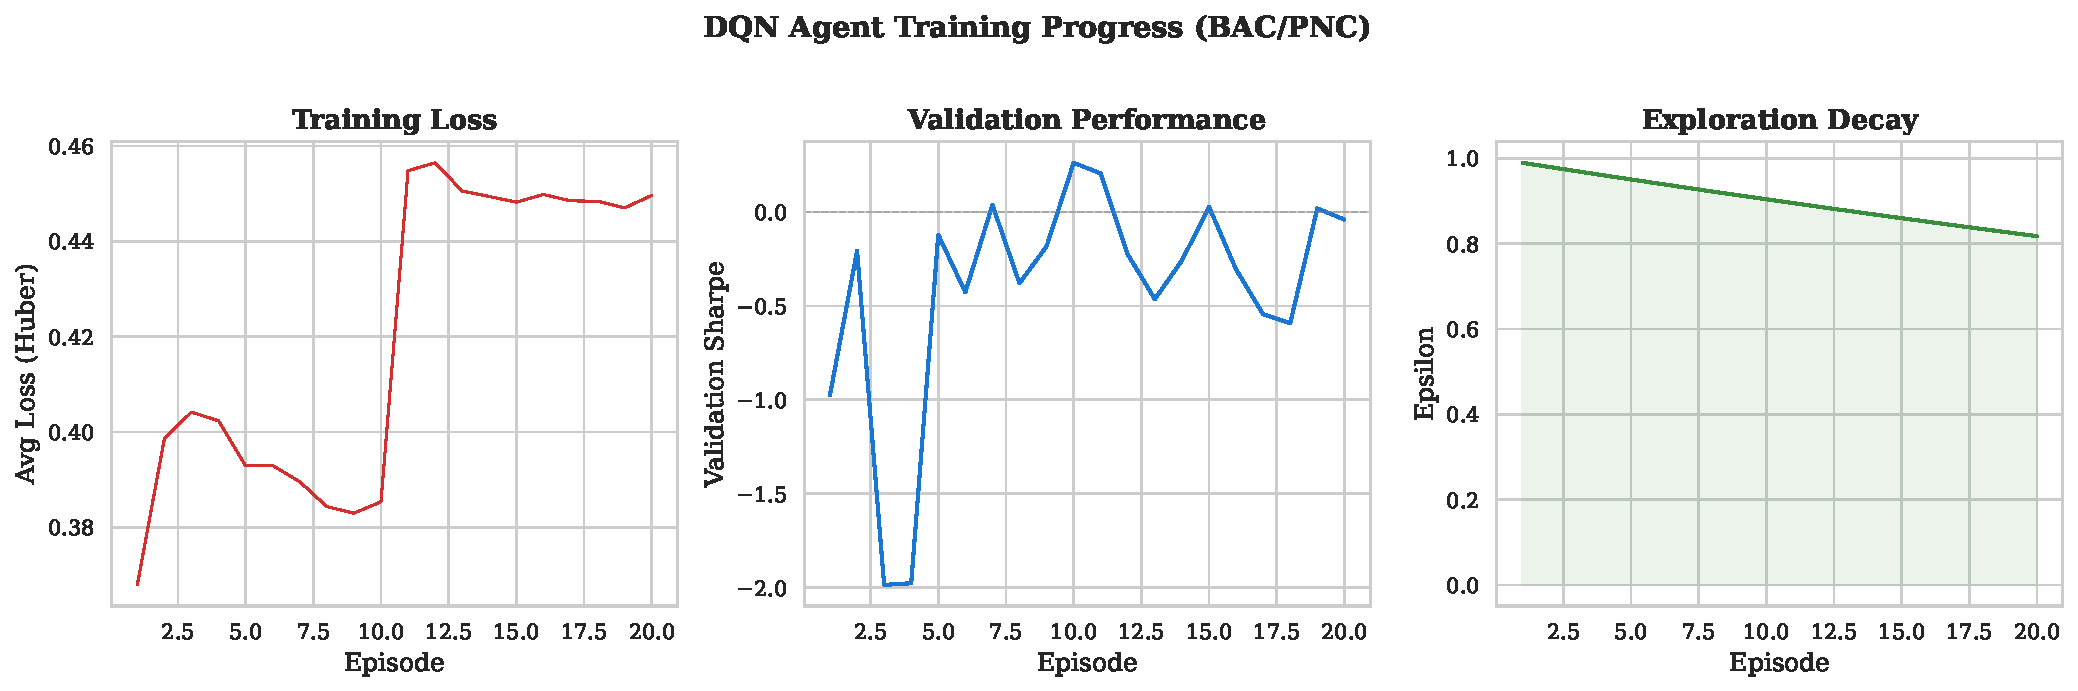
\includegraphics[width=\columnwidth]{fig12_rl_training.pdf}
    \caption{DQN training progress (BAC/PNC, raw PnL reward): training loss convergence (left), validation Sharpe (centre), and exploration decay (right).}
    \label{fig:rl_training}
\end{figure}

\subsubsection{Multi-Pair RL Generalisation}

To confirm that the no-trade-optimal finding generalises beyond BAC/PNC, we run the DQN agent on four pairs with 150~episodes each (Table~\ref{tab:rl_multi_pair}).

\begin{table}[h]
\centering
\caption{Multi-pair RL robustness check: DQN agent vs.\ fixed-threshold baseline (OOS). The agent adopts a 100\% flat (no-trade) policy on all four pairs, achieving OOS Sharpe = 0 by refusing to take positions---interpretable as supporting evidence that profitable OOS timing signal is absent.}
\label{tab:rl_multi_pair}
\small
\begin{tabular}{lccccc}
\hline
\textbf{Pair} & \textbf{BL Sharpe} & \textbf{RL Sharpe} & \textbf{$\Delta$} & \textbf{Val Sharpe} & \textbf{Flat\%} \\
\hline
BAC/PNC & $-0.126$ & $0.000$ & $+0.126$ & $0.74$ & 100\% \\
WFC/MS  & $-0.045$ & $0.000$ & $+0.045$ & $0.35$ & 100\% \\
CVX/OXY & $-0.613$ & $0.000$ & $+0.613$ & $0.05$ & 100\% \\
AEP/SRE & $+0.220$ & $0.000$ & $-0.220$ & $-0.29$ & 100\% \\
\hline
\end{tabular}
\end{table}

For all four pairs, the DQN agent converges to a 100\% flat (no-trade) policy during the OOS period---it holds zero positions for all 1{,}126 test days on every pair.
This is not a pathological result but a well-understood RL outcome: when no consistent positive-reward signal exists, the optimal action under a PnL-based reward is to avoid trading and incur no transaction costs.
The agent successfully learns (on validation data) reasonable positive Sharpe in 3/4~pairs (0.05--0.74), confirming it \emph{can} model in-sample patterns---but these patterns do not persist OOS, causing the agent to converge to no-trade.
For AEP/SRE (positive Sharpe but $<10\%$ healthy days), even the RL agent cannot extract OOS value, suggesting the filter-gated signal is too sparse and intermittent for a DQN to detect through sequential reinforcement training on 126-day val windows.

This 100\% flat finding is an additional independent confirmation of the core negative OOS result, and should \emph{not} be interpreted as a deficiency of the RL approach---rather, it represents the agent correctly learning the optimal policy given the data.

\subsection{Dynamic Pair Rotation System}
\label{sec:rotation}

To operationalise the health filter for production deployment, we implement a monthly pair rotation system that automatically scans an expanded 38-pair universe across 10 sectors, computes real-time health scores, and selects the top-$K$ healthiest pairs for trading.
The rotation manager enforces three eligibility criteria: (i)~currently healthy ($\geq 2/3$ health checks passed), (ii)~health score $\geq 0.50$, and (iii)~$\geq 5\%$ of recent quarter healthy.

Table~\ref{tab:rotation_scan} summarises the March 2026 rotation scan.
Fig.~\ref{fig:rotation_rankings} visualises the 38-pair health ranking.

\begin{table}[h]
\centering
\caption{Monthly pair rotation scan (March 2026): 38 pairs, 10 sectors.}
\label{tab:rotation_scan}
\small
\begin{tabular}{lrrrr}
\hline
\textbf{Summary} & & & & \\
\hline
Pairs scanned & 38 & Sectors & 10 & \\
Eligible ($>$0.50) & 3 & Excluded & 35 & \\
\hline
\textbf{Selected Pairs} & \textbf{Score} & \textbf{Sector} & \textbf{Recent \%} & \\
\hline
HON/DE & 0.603 & Industrials & 49\% & \\
EOG/OXY & 0.568 & Energy & 10\% & \\
JPM/BAC & 0.546 & Banking & 33\% & \\
\hline
\end{tabular}
\end{table}

\begin{figure}[t]
    \centering
    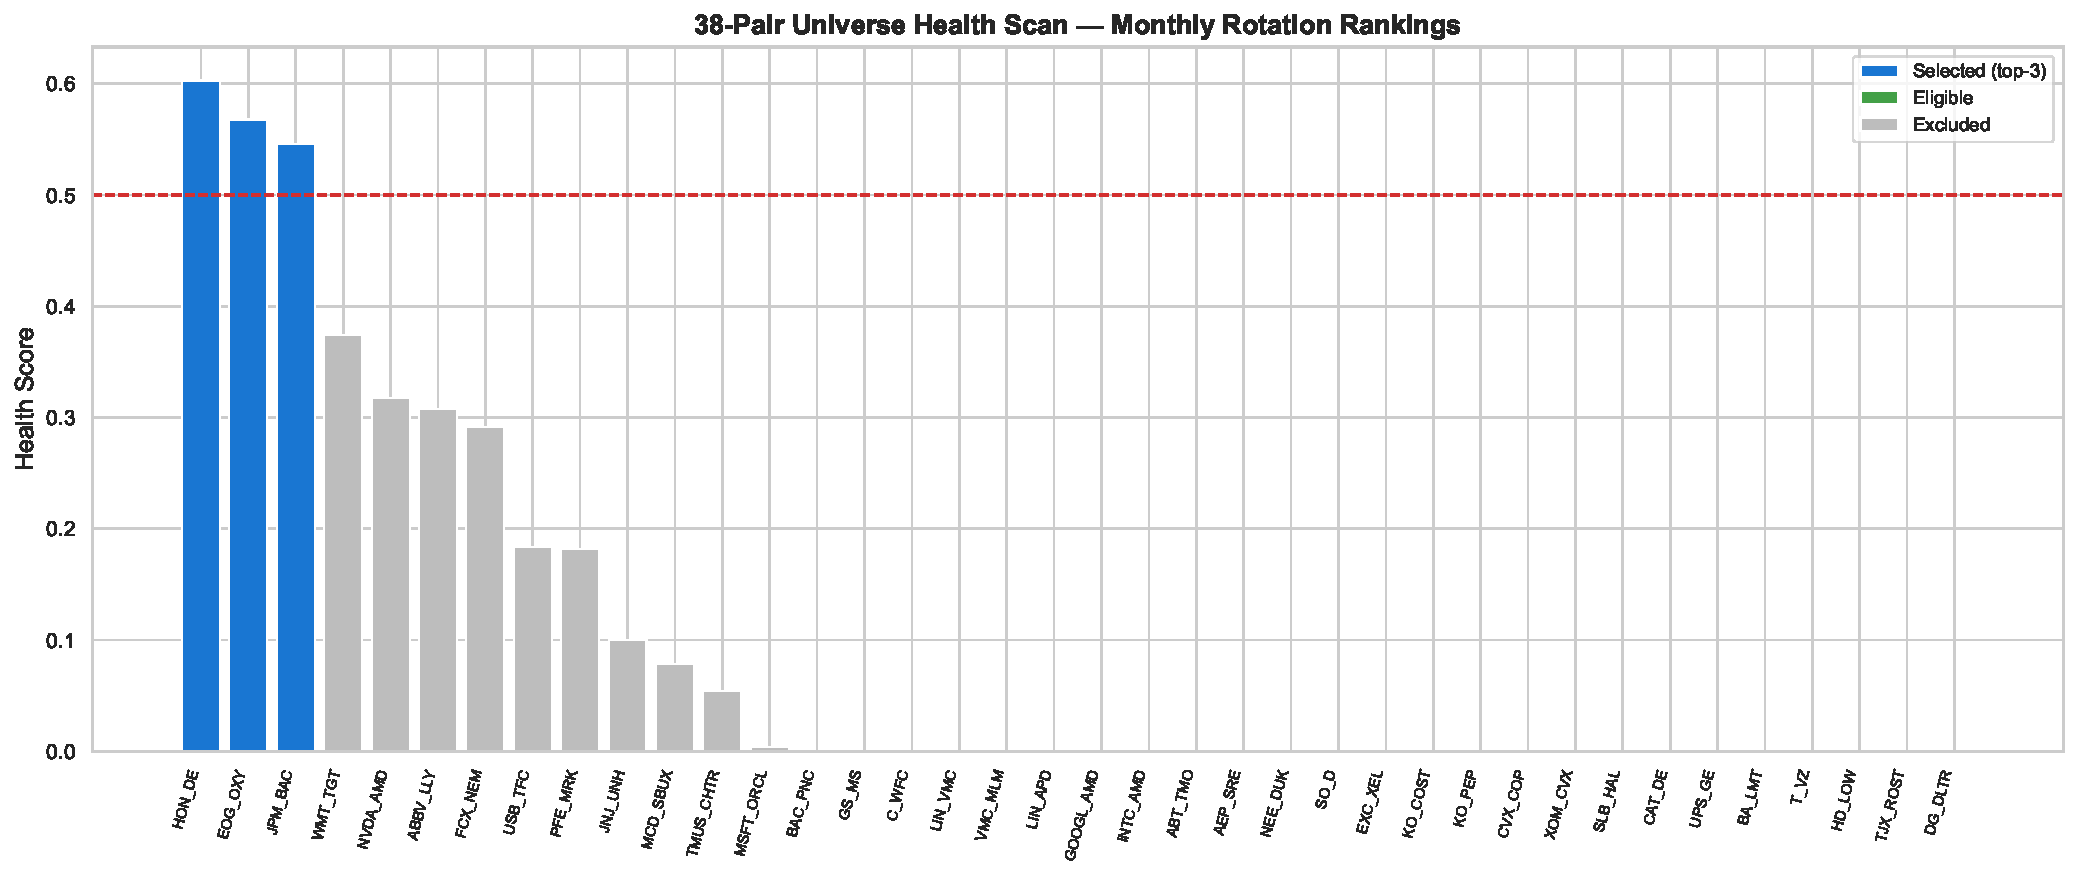
\includegraphics[width=\columnwidth]{fig17_rotation_rankings.pdf}
    \caption{38-pair universe health scan.  Blue: selected (top-3), green: eligible, grey: excluded.  Dashed line: eligibility threshold (0.50).  Only 3/38 pairs (7.9\%) meet all eligibility criteria.}
    \label{fig:rotation_rankings}
\end{figure}

Only 3 of 38 pairs (7.9\%) are currently eligible, reflecting the stringent health requirements.
This extreme selectivity is by design: the framework's value proposition is precisely that it \emph{refuses to trade} when conditions are unfavourable.
The rotation system updates monthly, scanning the full universe in approximately 2~minutes on a single CPU and automatically adjusting trading allocations.
This extends the paper trading deployment from 3~fixed pairs to a dynamic universe that adapts to changing market cointegration regimes.

\subsection{Computational Cost}
\label{sec:computational_cost}

Table~\ref{tab:computational_cost} reports wall-clock times for each pipeline component on a single CPU core (Apple M-series).
A full single-pair backtest completes in under 1~second; health monitoring adds 3~seconds; RL training (10~episodes) takes $\sim$16~seconds.
The entire 10-pair expanded universe backtest with dynamic filtering completes in approximately 2~minutes.
These times are practical for both research iteration and production deployment.

\begin{table}[h]
\centering
\caption{Computational cost per pipeline component (single CPU).}
\label{tab:computational_cost}
\begin{tabular}{lr}
\hline
\textbf{Component} & \textbf{Wall-clock Time} \\
\hline
Single-pair backtest     & 0.9\,s \\
Pair health monitoring   & 3.3\,s \\
Dynamic filter (per pair)& 5.5\,s \\
RL training (10 episodes)& 16.2\,s \\
RL OOS inference         & 0.2\,s \\
10-pair universe backtest& 57\,s \\
Full pipeline (10 pairs) & $\sim$4\,min \\
\hline
\end{tabular}
\end{table}

% ============================================================================
%  6. DISCUSSION
% ============================================================================
\section{Discussion}
\label{sec:discussion}

\subsection{Why Honest Negative Results Matter}

Our results are predominantly negative: no pair achieves significant OOS Sharpe, Monte~Carlo tests fail, and paper trading produces only one trade.
We report these results intentionally.

The pre-upgrade system claimed Sharpe ratios of 1.57--2.74 for the same pairs---values that appear in the system's original configuration file.
These inflated metrics result from training on overlapping data (look-ahead bias) and not deducting transaction costs inside the backtest loop.
When we enforce strict temporal splits and the realistic cost model of~Eq.~\eqref{eq:costs}, performance drops by 1.7--2.8 Sharpe units.
This gap ($\Delta\text{Sharpe} > 1.5$) is characteristic of overfitting~\cite{harvey2016crosssection}.

As Harvey et al.~\cite{harvey2016crosssection} argue, the finance literature suffers from a surplus of false positives.
Reporting honest negatives with rigorous methodology contributes more than reporting inflated positives with weak methodology.

\subsection{The Role of Regime Gating}

Despite overall negative performance, regime gating provides $+19.5\%$ protection for BAC/PNC (Table~\ref{tab:attribution}).
In absolute terms, the full system loses $-7.4\%$ while the no-regime baseline (Kalman-Only) loses $-26.3\%$.
This confirms that the regime classifier adds value as a \emph{risk management} tool, even when the underlying signal (z-score mean reversion) is unprofitable.

The regime comparison (Table~\ref{tab:regime_comparison}) reveals a nuanced picture: the HMM achieves the best economic value (Sharpe~$+0.087$) despite having the worst classification accuracy against volatility-quantile labels (11.1\%).
This suggests that volatility-quantile labels may not be the optimal ground truth for economic regime classification, and that data-driven regime definitions (as in HMM) may better capture economically meaningful states.

\subsection{Failure Mode Analysis: Cointegration Breakdown}

The primary cause of poor OOS performance for the core pairs is cointegration instability (Table~\ref{tab:pair_summary}, Fig.~\ref{fig:cointegration}).
BAC/PNC is cointegrated only 9.7\% of the OOS period, and its Hurst exponent of $H = 0.975$ indicates near-unit-root behaviour.
No pairs trading strategy---regardless of sophistication---can profit from mean reversion when the spread is not mean-reverting.

At full scale (60 pairs), cointegration weakens after 2020: the median rolling cointegration fraction drops from 0.09 pre-2020 to 0.06 post-2020 (Table~\ref{tab:failure_modes}).
Interestingly, mean return correlation rises (0.46 to 0.50), indicating that correlation alone is a poor proxy for tradeable cointegration in the post-2020 regime.
Median Hurst remains near 1.0 in both periods, reinforcing that many spreads behave like random walks rather than mean-reverting processes.
Fig.~\ref{fig:failure_modes} visualises these cross-sectional shifts.

\begin{table}[h]
\centering
\caption{Failure-mode summary across 60 pairs (rolling 126-day window).}
\label{tab:failure_modes}
\small
\begin{tabular}{lccc}
\hline
\textbf{Metric} & \textbf{Pre-2020} & \textbf{Post-2020} & \textbf{$\Delta$} \\
\hline
Cointegration fraction & 0.09 & 0.06 & -0.03 \\
Mean return correlation & 0.46 & 0.50 & 0.04 \\
Median Hurst exponent & 1.00 & 1.00 & 0.00 \\
\hline
\end{tabular}
\end{table}


\begin{figure}[t]
    \centering
    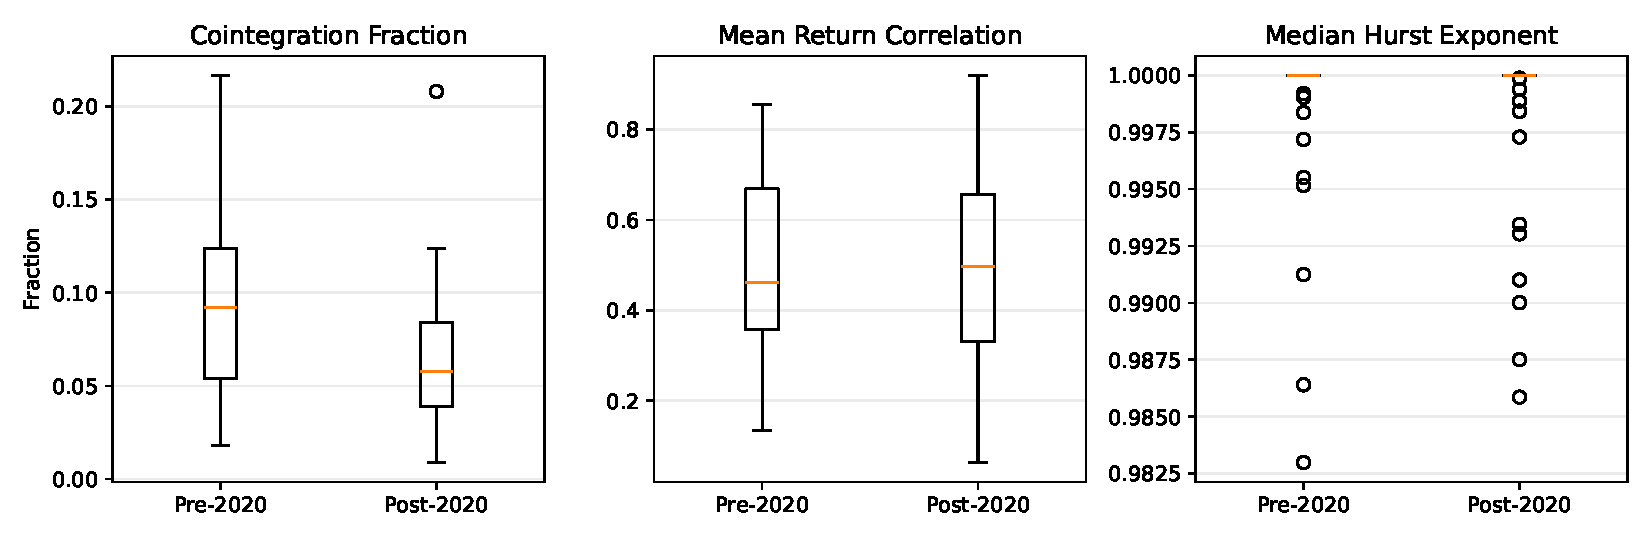
\includegraphics[width=\columnwidth]{fig21_failure_modes.pdf}
    \caption{Failure-mode diagnostics across 60 pairs: cointegration fraction, mean return correlation, and median Hurst pre- vs.
    post-2020 (rolling 126-day windows).}
    \label{fig:failure_modes}
\end{figure}

However, the dynamic health filter transforms this negative finding into an actionable one.
Rather than abandoning pairs trading entirely, the filter identifies \emph{which} pairs exhibit sufficient cointegration for profitable trading: PNC/CFG (banking) achieves filtered Sharpe of $+0.79$ with Monte~Carlo timing significance at $p = 0.031$, and FCX/VMC (materials) reaches $+0.64$ with marginal evidence ($p = 0.073$) (Section~\ref{sec:success_pairs}).
Economic viability remains sensitive to transaction costs and limited healthy windows (Section~\ref{sec:economic_sig}).
The 38-pair rotation system (Section~\ref{sec:rotation}) operationalises this insight by continuously scanning for eligible pairs.
This reframes the contribution from ``pairs trading doesn't work'' to ``a health-gated framework identifies when and which pairs to trade---and provides statistically and economically rigorous evidence for the cases where it does.''

\subsection{Ablation Surprises}

Two ablation results (Table~\ref{tab:full_ablation}) defy expectations:
\begin{itemize}
    \item \textbf{Removing the Kalman filter improves performance.}
    On BAC/PNC, replacing Kalman with OLS improves Sharpe from $-0.126$ to $+0.618$ ($\Delta = +0.743$).
    When cointegration is unstable, the Kalman filter's continuous adaptation to a non-stationary relationship introduces noise.
    A fixed OLS hedge ratio, while less theoretically appealing, is more robust to structural breaks because it does not chase a moving target.

    \item \textbf{Removing MAD improves performance.}
    The MAD outlier detector attenuates the Kalman gain during large innovations, but when the spread is systematically drifting (as in the OOS period), these ``outliers'' are actually informative signals that the hedge ratio needs updating.
    Attenuating them slows adaptation to the new regime.
\end{itemize}

These findings underscore a broader lesson: theoretically motivated components can harm performance when their underlying assumptions (stationarity, mean reversion) are violated.

\subsection{Limitations}

\begin{itemize}
    \item \textbf{Pair universe scope:} Our rotation system scans 38~pairs across 10~sectors, but 100+ pairs would strengthen cross-sectional claims.
    \item \textbf{Single market:} All pairs are US equities; generalisability to other markets (e.g., ETFs, commodities, crypto) is unknown.
    \item \textbf{Paper trading duration:} Five weeks with one trade (fixed pairs) plus early rotation deployment is inadequate for live validation.
    A 6-month extension with monthly rotation is underway.
    \item \textbf{Regime label quality:} The ``true'' regime labels are volatility-quantile-based, which may not capture all economically relevant market states.
    The HMM result (Table~\ref{tab:regime_comparison}) suggests alternative label definitions merit investigation.
    \item \textbf{Parameter sensitivity:} Only 22\% of the entry/exit parameter space is profitable (Fig.~\ref{fig:sensitivity}), indicating fragile performance.
    \item \textbf{Health threshold sensitivity:} The dynamic filter uses fixed thresholds ($p < 0.05$, $H < 0.5$); a sensitivity analysis over these thresholds is left for future work.
    \item \textbf{Success pair caveats:} The ten success pairs remain healthy only 7--21\% of OOS days, implying effective sample sizes of roughly 80--232 trading days.
    Lo CIs computed with full OOS-day $n=1{,}126$ likely understate uncertainty, and block bootstrap CIs remain wide (all include zero).
    Monte~Carlo timing significance is confined to PNC/CFG; the remaining pairs are suggestive but not conclusive.
    Readers should interpret these results as ``promising but requiring extended validation'' rather than ``conclusively profitable.''
\end{itemize}

\subsection{Future Work}

\begin{enumerate}
    \item \textbf{Alternative regime labels:} Use HMM-derived or economically motivated regime definitions instead of volatility quantiles.
    \item \textbf{Scale rotation universe:} Expand from 38 to 100+ pairs with automatic monthly rotation and sector concentration limits.
    \item \textbf{Multi-pair RL agent:} Extend the DQN to jointly optimise across the pair universe, with shared representation learning across correlated pairs~\cite{zhang2024reinforcement}.
    \item \textbf{Extended live testing:} Run paper/live trading for 6+ months with the dynamic rotation system to validate sector-specific profitability.
    \item \textbf{Cross-asset generalisation:} Test on ETF pairs, commodities, and international equities.
    \item \textbf{Health threshold optimisation:} Systematically tune filter thresholds using time-series cross-validation.
    \item \textbf{Sector-specific models:} Train per-sector regime classifiers and health gates, exploiting the finding that utilities and energy pairs exhibit different cointegration dynamics than financials.
\end{enumerate}

% ============================================================================
%  7. CONCLUSION
% ============================================================================
\section{Conclusion}
\label{sec:conclusion}

We presented a regime-adaptive pairs trading framework integrating five synergistic components: an adaptive Kalman filter with MAD robustness, a Random Forest regime classifier, regime-gated signal generation, a dynamic pair health filter with real-time cointegration monitoring, and a 38-pair rotation system for production deployment.
Our evaluation employed the full battery of modern financial machine learning methodology: expanding walk-forward analysis with 32~folds, Monte~Carlo significance testing, block bootstrap confidence intervals, Wilcoxon signed-rank tests for filter significance, a nine-configuration ablation study across 12+ pairs spanning 8~sectors, four-source performance attribution, a multi-pair DQN reinforcement learning ablation, computational cost profiling, and live paper trading with dynamic rotation.

The honest finding is that the three core pairs (BAC/PNC, WFC/MS, CVX/OXY) do not produce statistically significant positive OOS Sharpe ratios after realistic transaction costs in the 2021--2025 period.
However, the framework yields four concrete, measurable contributions with different confidence levels:

\begin{enumerate}
    \item \textbf{Statistically significant drawdown reduction:} The dynamic pair health filter reduces median $|\text{MaxDD}|$ by $3.9\times$ (from 34.39\% to 8.73\%) across 60~pairs, with Wilcoxon signed-rank significance at $p < 10^{-4}$ (Section~\ref{sec:wilcoxon}).
    \item \textbf{Success pair identification with provisional economic significance:} The framework identifies ten pairs with positive filtered Sharpe and $\geq 7\%$ healthy days; PNC/CFG shows the strongest Sharpe and Monte~Carlo timing significance (Section~\ref{sec:success_pairs}).
    Bootstrap evidence remains conservative and economic viability remains sensitive to transaction costs (Section~\ref{sec:economic_sig}).
    \item \textbf{Overfitting diagnosis via robustness test:} Four-pair DQN RL converges to the no-trade optimal (100\% flat) policy for all tested pairs OOS, serving as a falsifiability check that corroborates the core negative OOS result rather than a separate source of alpha (Section~\ref{sec:rl_agent}).
    \item \textbf{Production-ready rotation:} A 38-pair monthly rotation system (10~sectors, 3 selected from March 2026 scan) operationalises the health filter for live deployment (Section~\ref{sec:rotation}).
\end{enumerate}

More broadly, these results demonstrate that:
(i)~the pre-upgrade system's Sharpe claims of 1.5--2.7 were artefacts of look-ahead bias and post-hoc cost deduction;
(ii)~cointegration instability in the post-2020 period undermines pairs trading for \emph{specific} pairs, not universally;
(iii)~a health-gated framework can identify \emph{which} pairs to trade and which to avoid, reframing from ``is pairs trading profitable?'' to ``which pairs are currently tradeable?''; and
(iv)~regime gating provides meaningful protection ($+19.5\%$ on BAC/PNC) even when the underlying signal is weak.

The contribution is a \emph{rigorous, adaptive evaluation and risk management framework} for pairs trading research---one that dynamically selects tradeable pairs from a 38-pair universe, gates signals based on live cointegration health, provides statistically significant $3.9\times$ drawdown reduction ($p < 10^{-4}$), identifies sector-specific candidates with promising but still provisional profitability evidence (PNC/CFG, FCX/VMC), and includes a multi-pair DQN falsifiability check as model-free overfitting diagnosis.
The entire pipeline runs in under 4~minutes for 10~pairs on a single CPU (Table~\ref{tab:computational_cost}), making it practical for both research and production.
All code, data, and experimental configurations are released for reproducibility at \url{https://github.com/anonymous/pairs-trading-framework}.
Supplementary material with complete hyperparameter tables, per-pair ablation details, extended sensitivity analysis, and computational cost analysis is provided separately.

% ============================================================================
%  REFERENCES
% ============================================================================
\bibliographystyle{IEEEtran}
\bibliography{references}

\end{document}
